\documentclass{PoS}

\usepackage{ptdr-definitions}

\providecommand{\JETPHOX} {{\textsc{JetPhox}}\xspace} 
\providecommand{\OPENLOOPS} {{\textsc{OpenLoops}}\xspace} 
\providecommand{\NLOJETPP} {{\textsc{NLOJet++}}\xspace} 
\providecommand{\NJET} {{\textsc{NJet}}\xspace} 
\providecommand{\BLACKHAT} {{\textsc{BlackHat}}\xspace} 
\providecommand{\HEJ} {{\textsc{HEJ}}\xspace} 
\providecommand{\kts}{\ensuremath{k_{\mathrm{t}}}\xspace}
\def\as{\ensuremath{\alpha_\mathrm{S}}\xspace}
\def\asq{\ensuremath{\alpha_\mathrm{S}(Q)}\xspace}
\providecommand{\alpsmz}{\ensuremath{\alpha_\mathrm{S}(M_\mathrm{Z})}\xspace}
\providecommand{\alpsq}{\ensuremath{\alpha_S(Q)}\xspace}
\providecommand{\dphi}{\ensuremath{\Delta\phi_\text{dijet}}\xspace}
\providecommand{\ptmax}{\ensuremath{\pt^{\text{max}}}\xspace}
\providecommand{\PYTHIAS} {{\textsc{pythia6}}\xspace}
\providecommand{\PYTHIAE} {{\textsc{pythia8}}\xspace}
\newcommand{\AMCATNLO} {a{\textsc{mc@nlo}}\xspace}
\newcommand{\GOSAM} {{\textsc{GoSam}}\xspace}

\title{Jet and photon physics in pp collisions at the LHC}

\ShortTitle{Jet and photon physics in pp collisions at the LHC}

\author{\speaker{ Vitaliano Ciulli }% %\thanks{} \\ Dipartimento di Fisica, Universit\`a di Firenze and Istituto
Nazionale di Fisica Nucleare, Sezione di Firenze, via G. Sansone 1, 50019 Sesto Fiorentino, Italy \\ E-mail:
\email{vitaliano.ciulli@fi.infn.it}} \author{on behalf of the ALICE, ATLAS, CMS and LHCb collaborations}

\abstract{Jets and photons production in proton-proton collisions at the Large Hadron Collider at CERN are key processes
  to test predictions of Quantum Chromodynamics and constraint the parton distribution functions of the proton. In this
  paper the most recent measurements from the LHC Collaborations are reviewed.}

\FullConference{Fourth Annual Large Hadron Collider Physics\\ 13-18 June 2016\\ Lund, Sweden}

\begin{document}
`
\section{Introduction}

Quantum Chromodynamics (QCD) is the fundamental theory describing strong interactions among partons, \ie quarks and
gluons. Jets and photons production in proton-proton collisions at the Large Hadron Collider (LHC) at CERN are key processes to test predictions of
perturbative QCD (pQCD) over a wide region in phase space, and constraint the parton distribution function (PDF) or the
proton. They are also among the main backgrounds to new physics searches and therefore needs to be measured with the
highest possible precision to allow discovering the tiniest deviations between data and theory.

The LHC collaborations, ALICE~, ATLAS~\cite{Aad:2008zzm}, CMS~\cite{Chatrchyan:2008aa} and LHCb, performed
measurements of inclusive jet production, multi-jets production, jet properties and photon and diphoton production. 
In the following we will review the most recent measurements.

\section{Jet Physics}

Jets are usually reconstructed with the anti-\kts algorithm~\cite{Cacciari:2008gp} with different values for the distance parameter $R$.
ATLAS uses topological clusters~\cite{Lampl:2008zz} of cells in the calorimeter as input objects. 
In CMS and LHCb, the particle-flow (PF) event algorithm~\cite{CMS:2009nxa}
first reconstructs and identifies each individual particle with an optimised
combination of information from the various elements of the detector. Next, these PF objects are used as input to the jet
reconstruction algorithm. ALICE uses both tracks and energy deposits in the
Electromagnetic Calorimeter to reconstruct jets in the region $|\eta|<0.9$.

The main experimental difficulties are the jet energy calibration and resolution estimate and the subtraction of pileup
effects. Additional proton-proton interactions (pileup) produce unwanted calorimetric energy depositions and additional
tracks. Different strategies have been developed to subtract these effect depending on the jet recontruction.

The results are usually compared to fixed-order predictions at NLO precision, complemented with electroweak (EW) corrections, and to predictions of
various Monte Carlo (MC) event generators that combine leading-order (LO) or next-leading-order (NLO) pQCD with the modeling of parton
showers (PS), hadronisation (HAD) and multiparton interactions (MPI).
Fixed-order parton-level calculations, to be compared with measurement, must be complemented with corrections for nonperturbative
(NP) effects that involve the modeling of HAD and MPI, which are obtained from MC programs. 

Inclusive jet production measurements have been performed with data collected at different centre-of-mass energies, ranging from 2.76 GeV to 13 TeV. 
Using 13 TeV data collected in 2015, the CMS experiment measured the double-differential inclusive jet
cross section as a function of the jet \pt and absolute jet rapidity $|y|$.\cite{Khachatryan:2016wdh}. The data samples correspond to
an integrated luminosity of 71\pbinv. During data collection the LHC operated with a $50\unit{ns}$ bunch spacing and the
average number of pileup interactions observed in these data is ${\approx}19$.   

Figure~\ref{fig:crossSection} shows the double-differential inclusive jet cross section measurements,
presented as a function of \pt for seven $|y|$ ranges, after
unfolding for detector effects, using the anti-\kts algorithm with $R =
0.7$ and $0.4$, respectively. The measurements are compared to the predictions from \POWHEG~\cite{Alioli:2010xa}
matched to \PYTHIAE~\cite{Sjostrand:2007gs} PS. The data are remarkably consistent with the predictions over a wide range of jet \pt from 114\GeV up to
2\TeV.

\begin{figure*}[htbp] \centering
  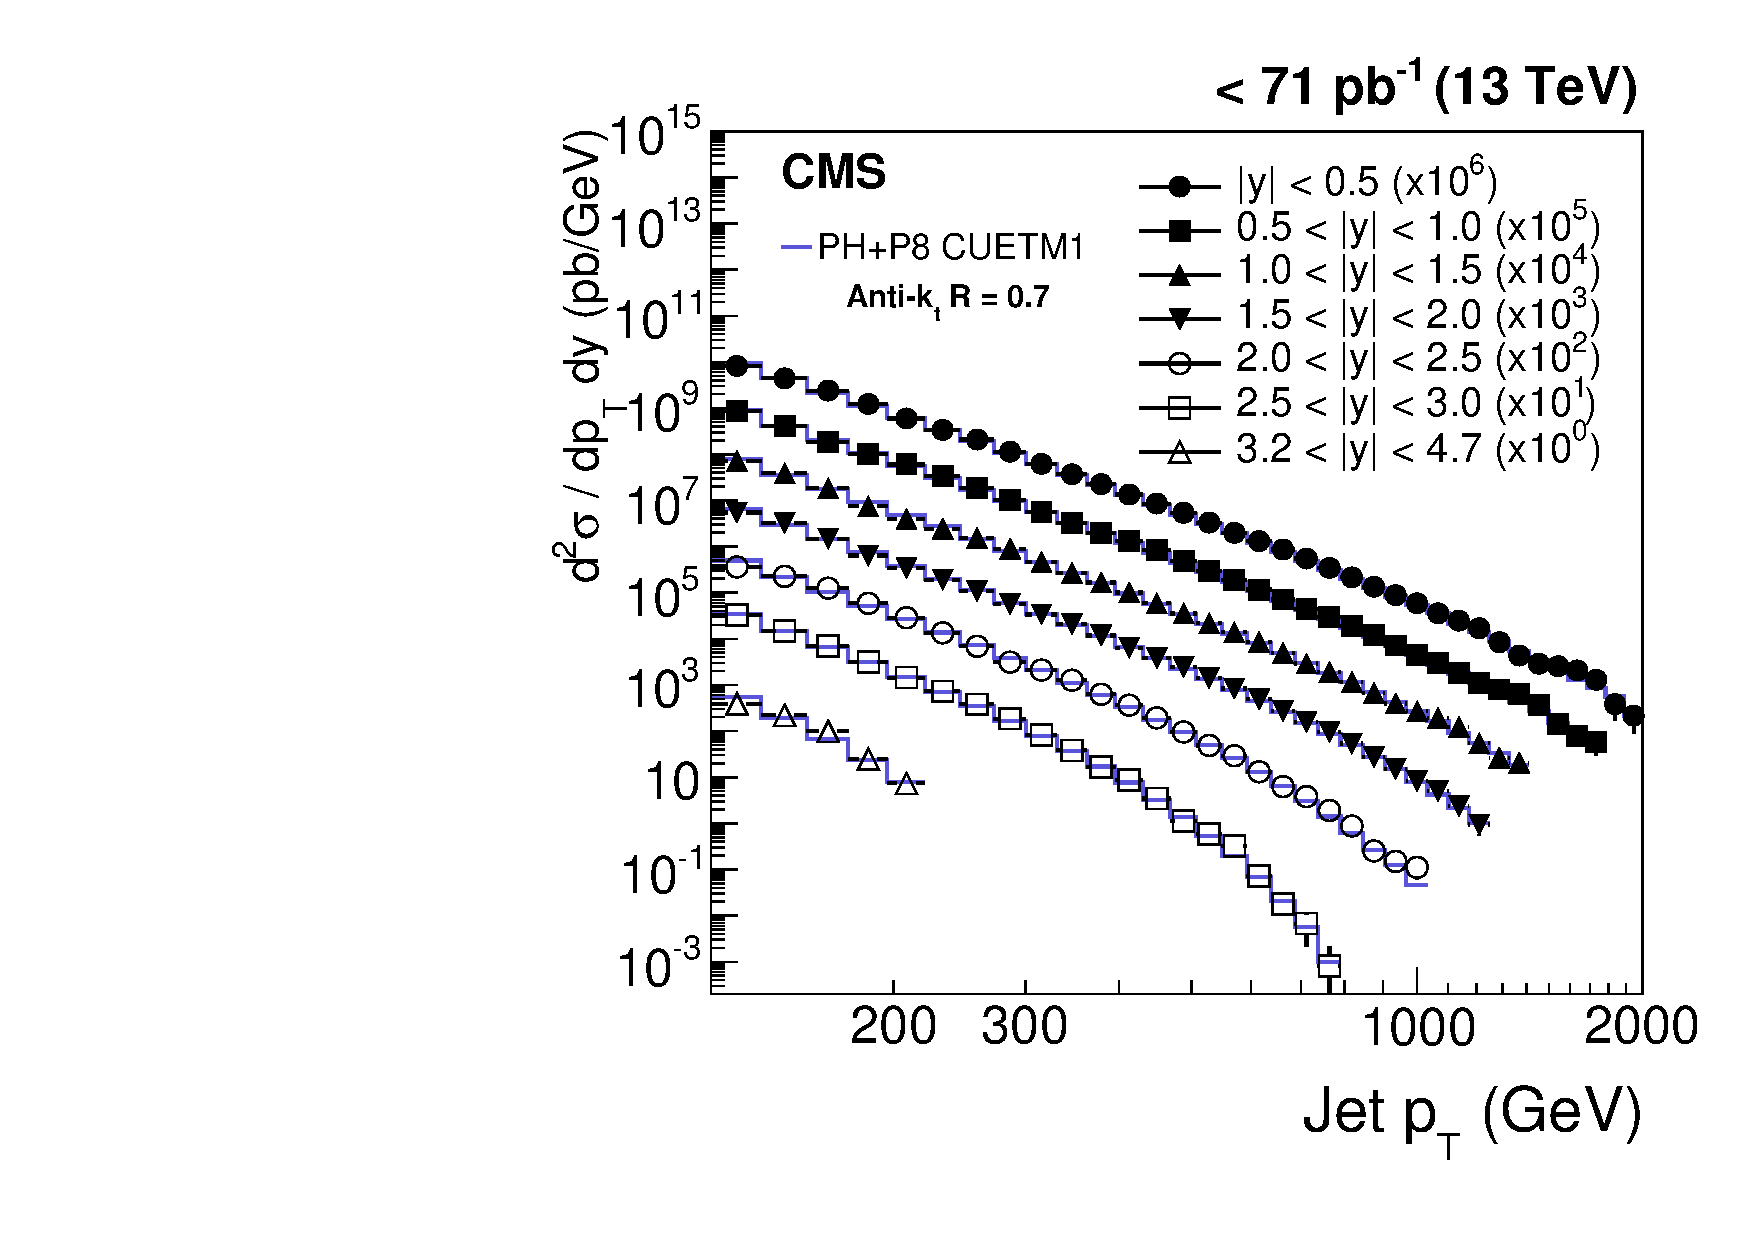
\includegraphics[width=0.48\textwidth]{Figure1-a.pdf}
  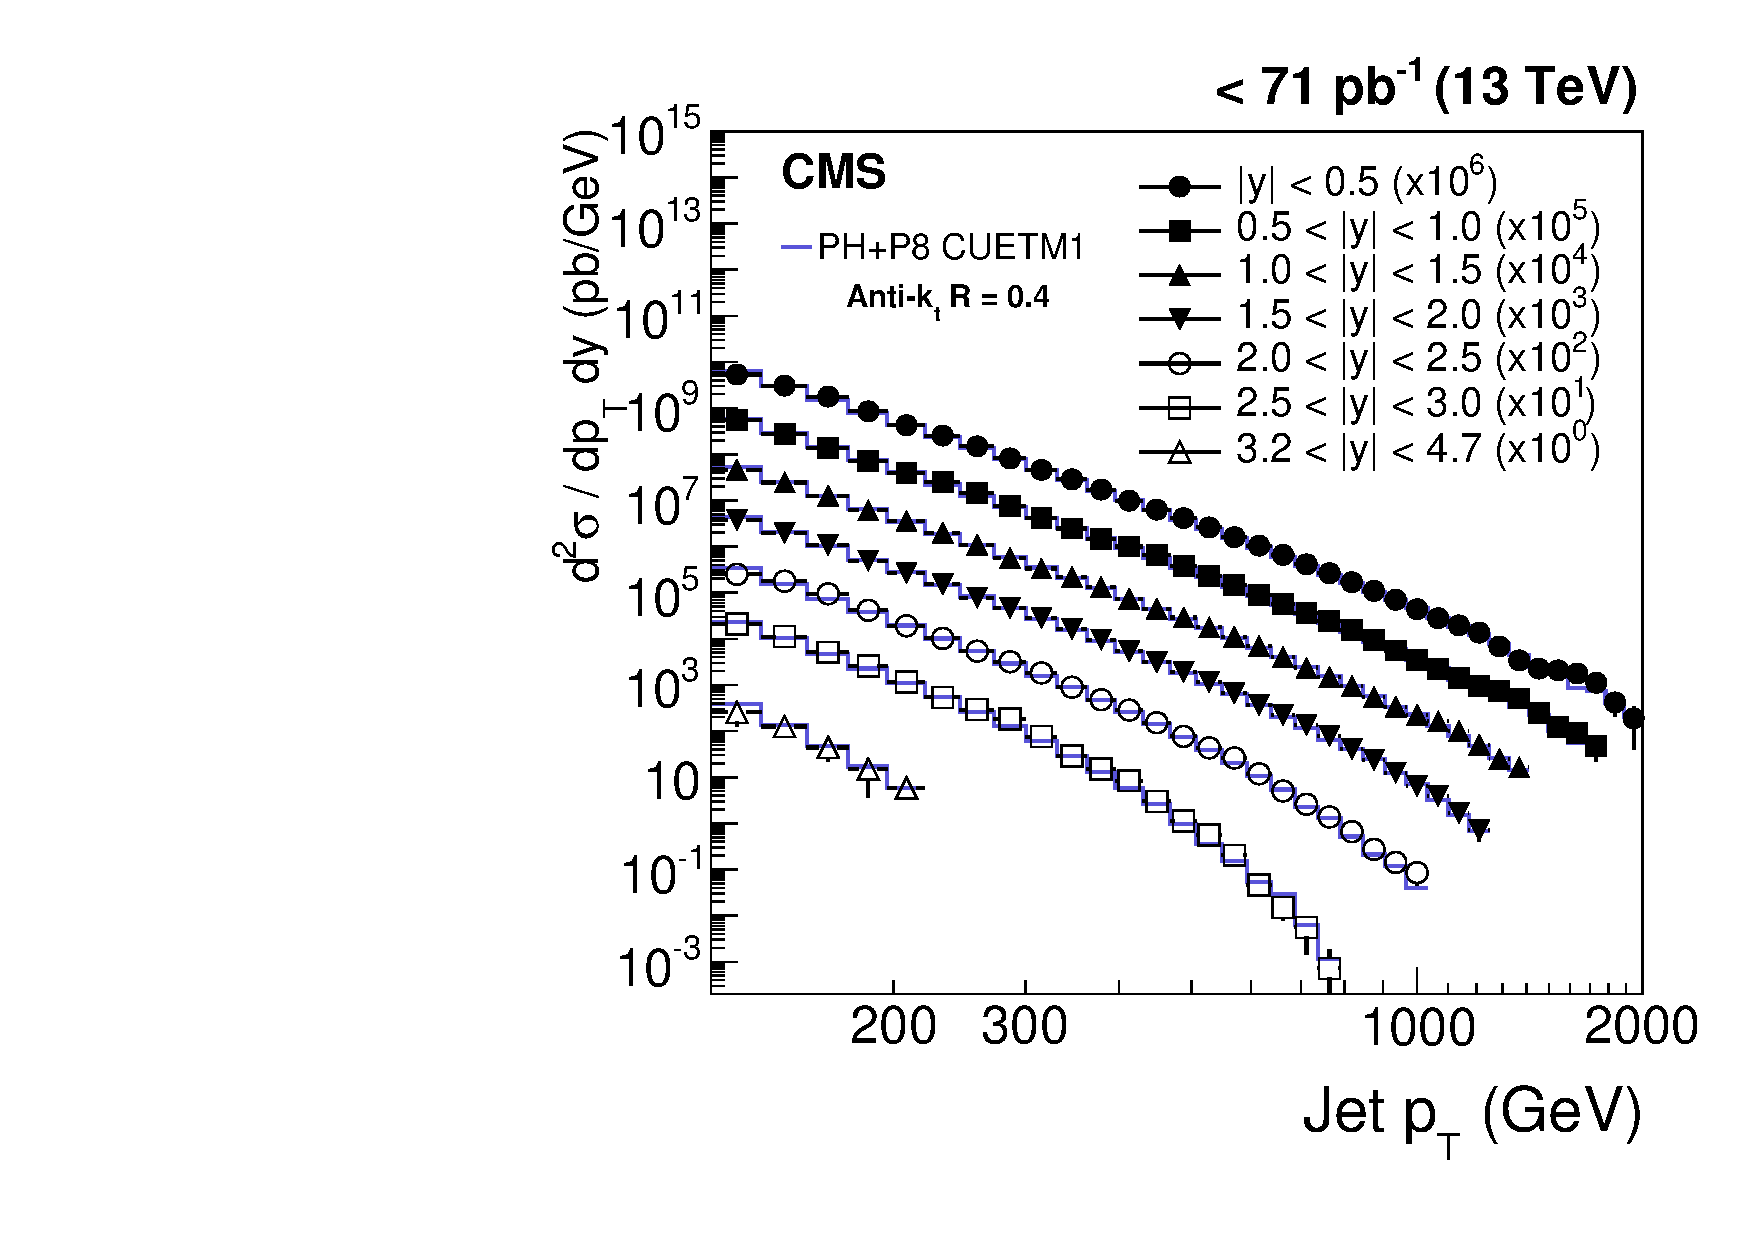
\includegraphics[width=0.48\textwidth]{Figure1-b.pdf}
  \caption{Double-differential inclusive jet cross section as function of jet \pt at 13 TeV. Data (points) and
predictions from \POWHEG + \PYTHIAE with tune CUETM1 (line) are shown. Jets are clustered with the anti-\kts
algorithm with $R = 0.7$ (left) and $0.4$ (right).}
  \label{fig:crossSection}
\end{figure*}

Results are also compared to the \NLOJETPP~\cite{Nagy:2003tz} predictions using the CT14 PDF set~\cite{Dulat:2015mca}, corrected for NP and EW effects.
The ratios of data over the \NLOJETPP predictions are shown in Fig.~\ref{fig:ratio_CT14} for the rapidity region
$|y|<0.5$, but the same trend is observed in all the rapidity ranges. The relatively poor agreement for $R = 0.4$ might
be due to parton-shower and soft-gluon resummation contributions, which are missing in fixed-order calculations, or to
higher-order effects. 

\begin{figure*}[htbp]
  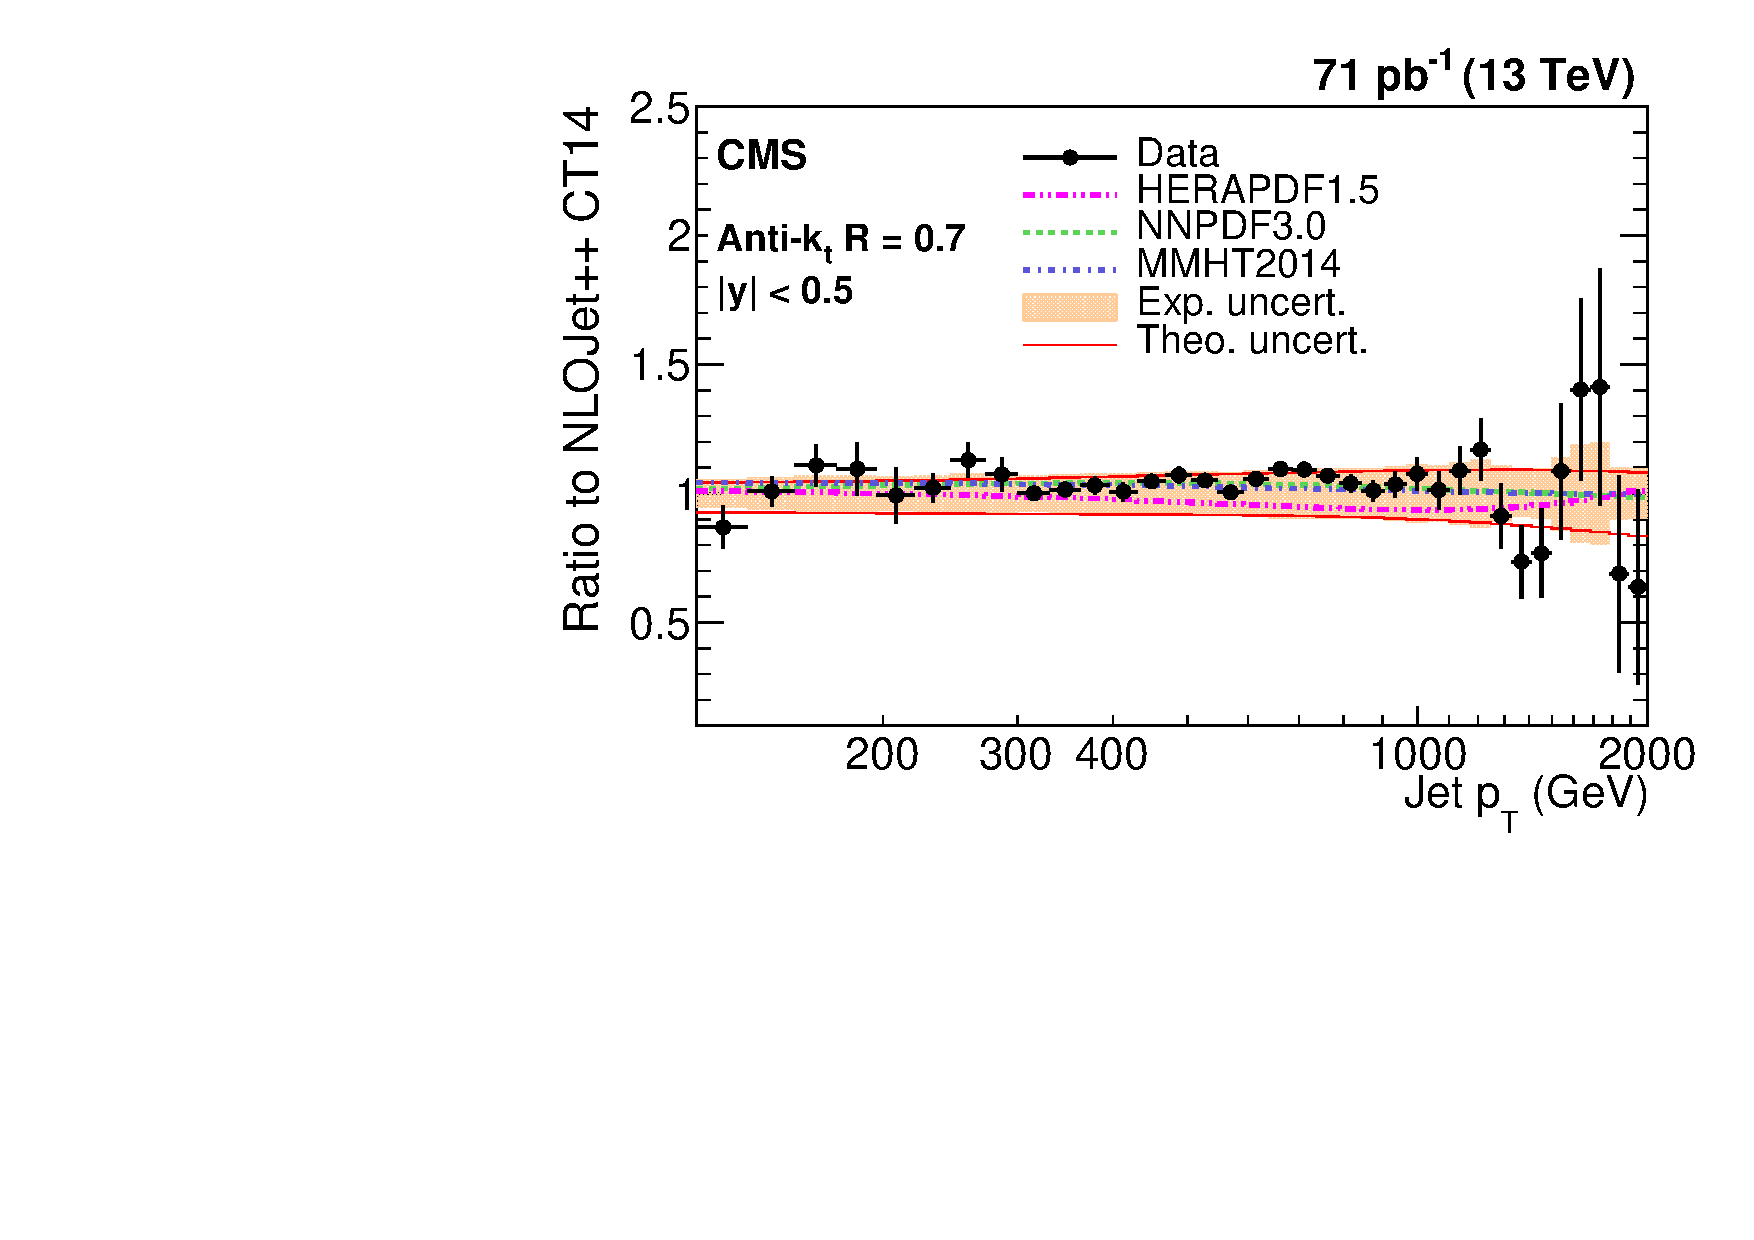
\includegraphics[width=0.48\textwidth]{Figure2-a.pdf}
  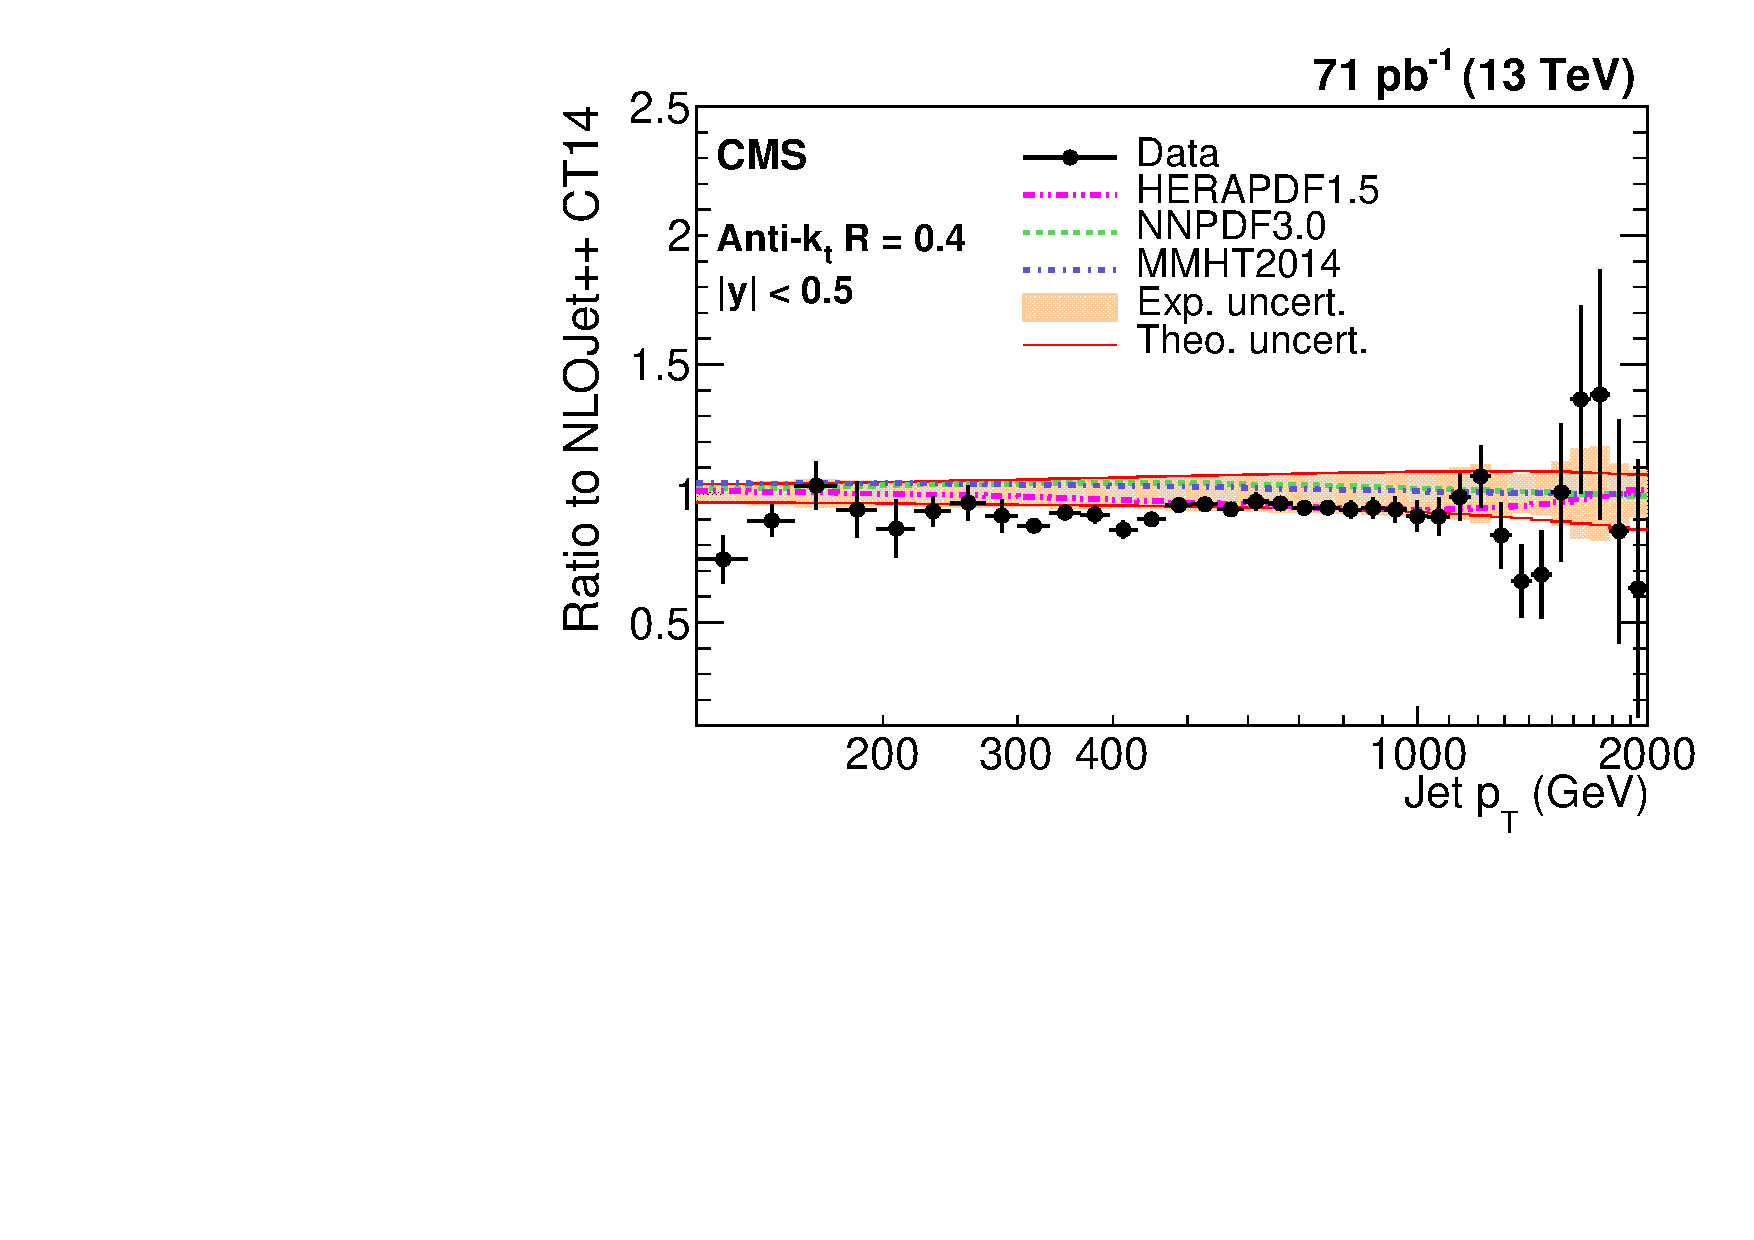
\includegraphics[width=0.48\textwidth]{Figure2-b.pdf}
  \caption{Ratio of measured values to theoretical prediction from \NLOJETPP using the CT14 PDF set and corrected for
the NP and EW effects. Predictions employing three other PDF sets are also shown for comparison. Jets are
clustered with the anti-\kts algorithm with a distance parameter of
0.7 (left) and 0.4 (right). The error bars correspond to the statistical
uncertainties of the data and the shaded bands to the total experimental systematic uncertainties.}
  \label{fig:ratio_CT14}
\end{figure*}

The CMS collaboration has also recently made available new results for the double-differential inclusive jet cross section at 8
\TeV~\cite{CMS:2015haa} and 2.76 \TeV~\cite{Khachatryan:2015luy}. In the measurement at 8 \TeV, the ratio to the
cross section at 7 \TeV is also presented. A good agreement is observed in general between data and predictions, but for high
transverse momentum some discrepancies is present, in particular in the region $1.0 < \abs{y} < 1.5$, shown in
Figure~\ref{fig:ratio8to7}.

\begin{figure*}[hbpt]
  \centering
  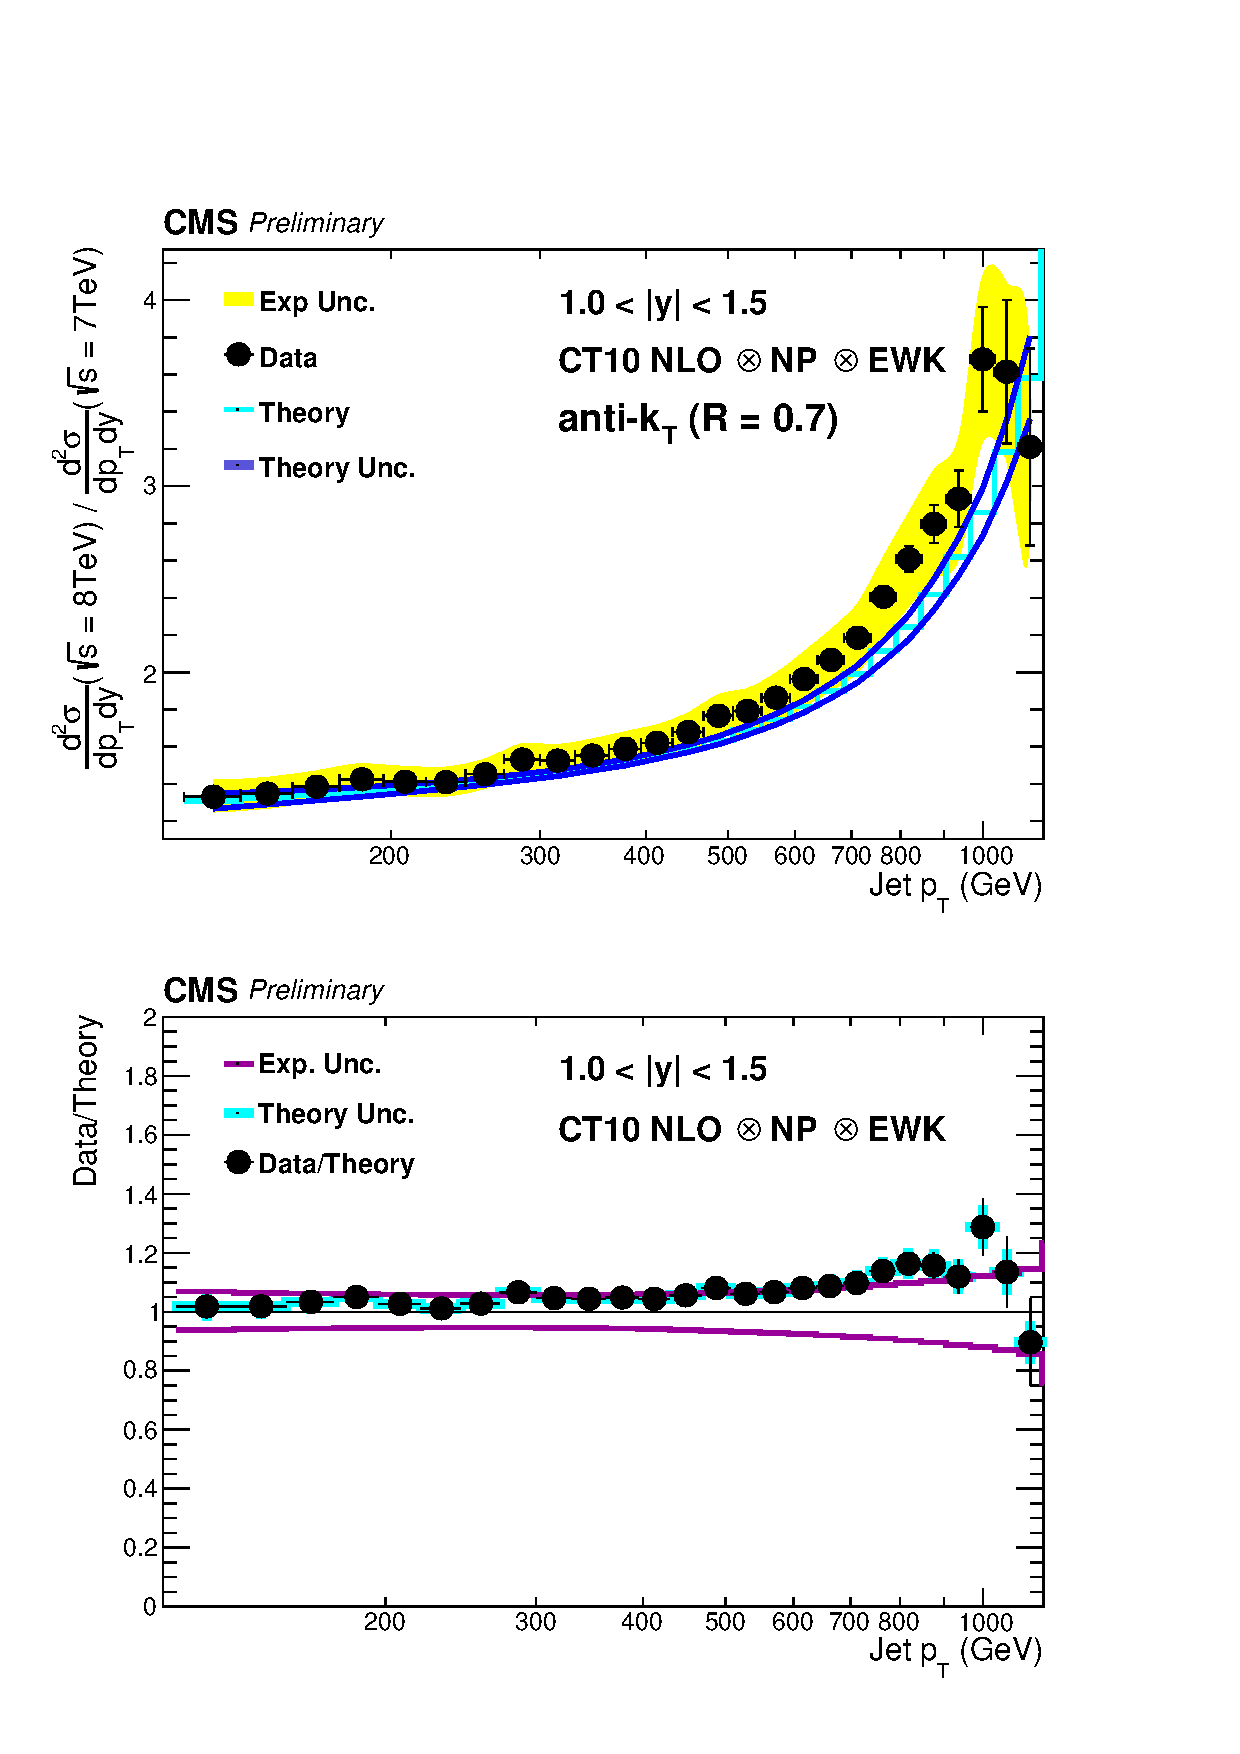
\includegraphics[width=0.6\textwidth]{Figure3.pdf}
  \caption{Ratio of double-differential inclusive jet cross sections
    between $\mathrm{\sqrt{s}=8}$\TeV and $\mathrm{\sqrt{s}=7}$\TeV
    for rapidity bins $1.0 < |y| < 1.5$. In the top plots the yellow band shows the total
    experimental uncertainty, accounting for the correlation between
    different energies, and the theoretical prediction for the CT10
    PDF set is overlaid. The bottom plot shows the ratio of the measured
    cross section ratio to its theoretical prediction, with the
    experimental uncertainty shown as a full line band, and
    theoretical uncertainties as a shaded band.}
  \label{fig:ratio8to7}
\end{figure*}

The inclusive jet cross section at 8 \TeV is also important by iteself for contraining the PDFs, in particular the gluon
one, as it is shown in Figure~\ref{fig:pdf}, where the measurement is combined with the HERA
data\cite{Abramowicz:2015mha} using the HERAPDF method~\cite{Aaron:2009aa} 
\begin{figure}[h]
\center
   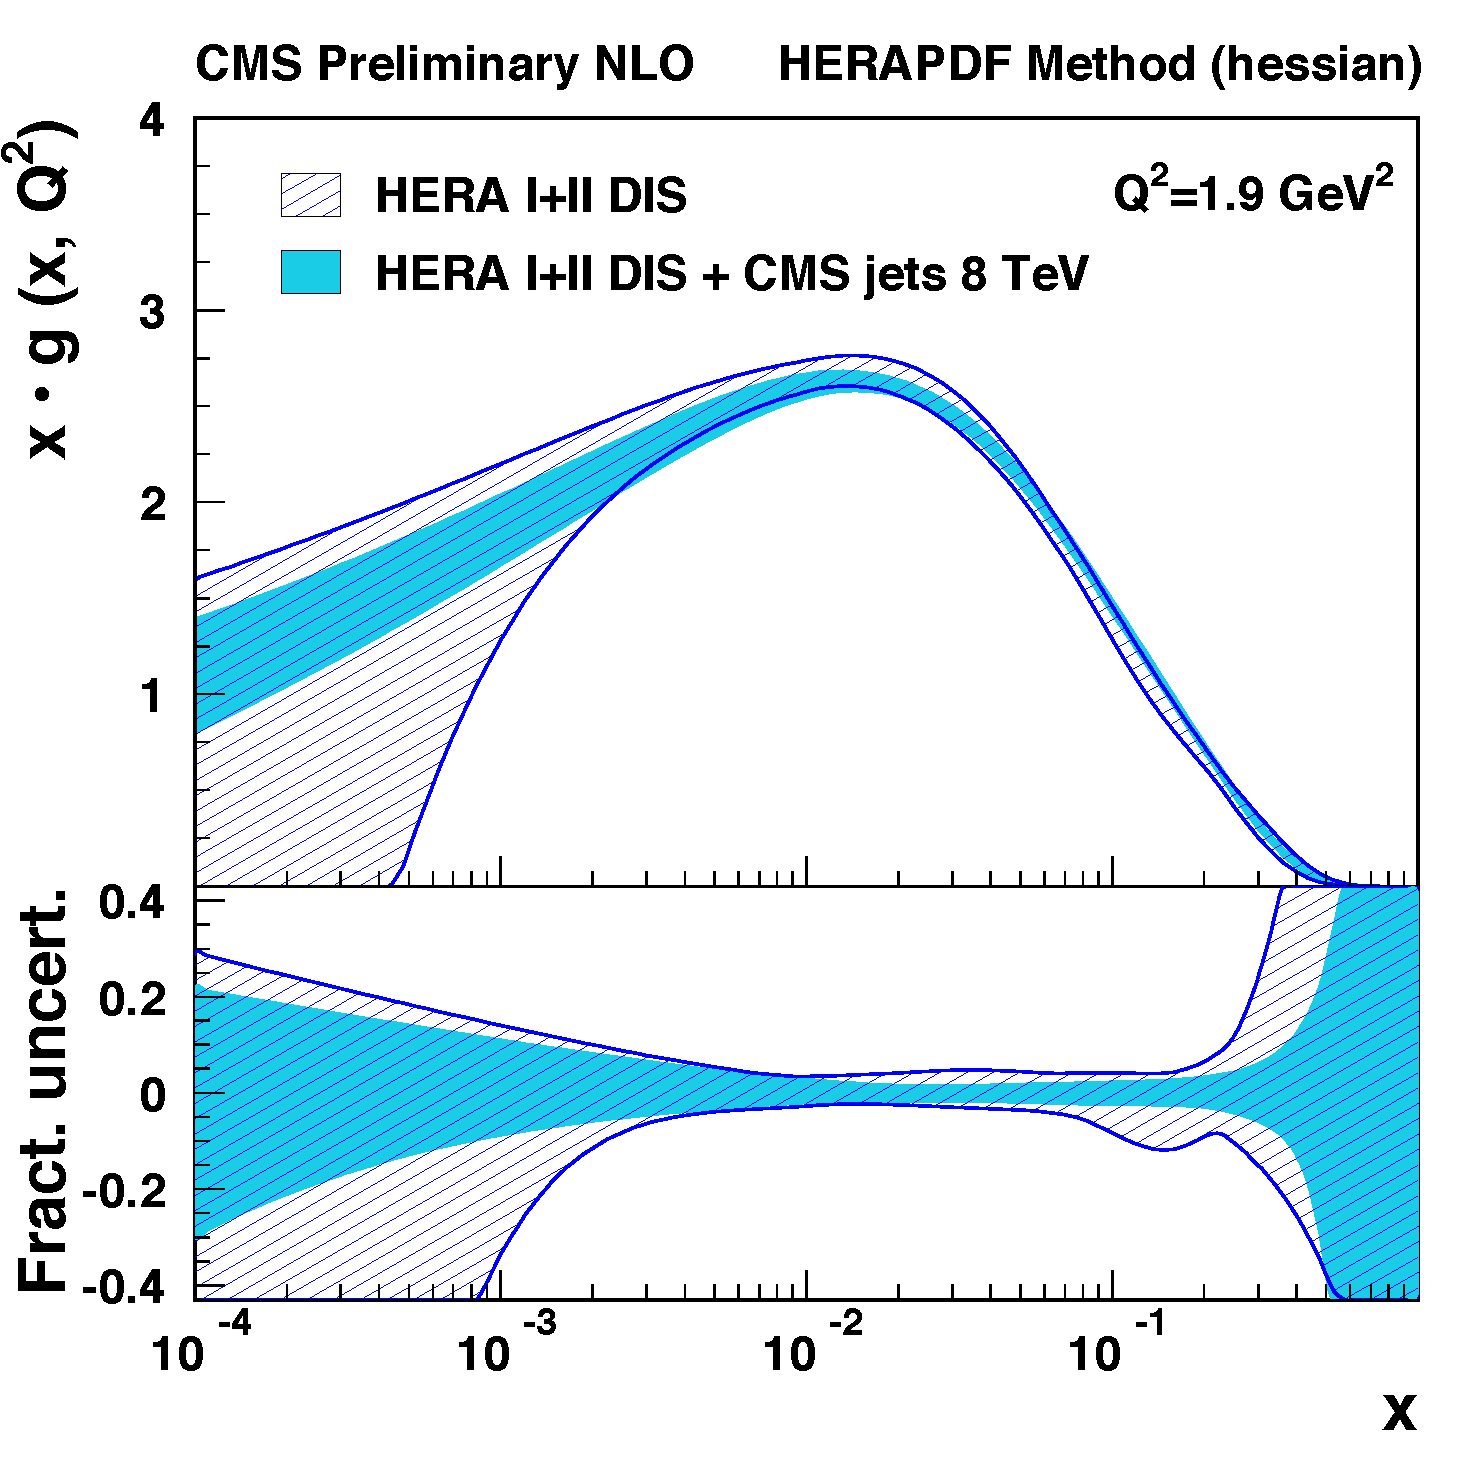
\includegraphics[width=0.6\textwidth]{Figure3b.pdf}
\setlength{\unitlength}{1cm}
\caption{Distributions of gluon as functions of $x$ at the starting scale
  $Q^2=1.9$\GeV$^2$. The results of the fit to the HERA
  data and inclusive jet measurements at 8\TeV (shaded band), and to
  HERA only (hatched band) are compared with their total
  uncertainties, as determined by using the HERAPDF method. In the
  bottom panels the fractional uncertainties are shown.}
\label{fig:pdf}
\end{figure}
%where the effect of the measurement is shown by combining it with the HERAPDF.
Furthermore the strong coupling constant \as is extracted from the measurement at 8 \TeV, using for the calculation the CT10 NLO PDF
set~\cite{Lai:2010vv}, which is found to provide the best agreement with data.
With the entire probed \pt range and six different rapidity bins, the best fitted value is found to be $\alpsmz =
0.1164^{+0.0060}_{-0.0043}$, which is compatible with the best current world average $\alpsmz =
0.1185\pm0.0006$~\cite{Agashe:2014kda}. The running of \asq, measured for nine different values of renormalization scale 
between 86\GeV and 1.5\TeV, is in good agreement with previous experiments and extends the measurement to the highest
values of the renormalization scale, as shown in Figure~\ref{fig:AlphasRun}.
\begin{figure*}[hbpt]
  \centering
 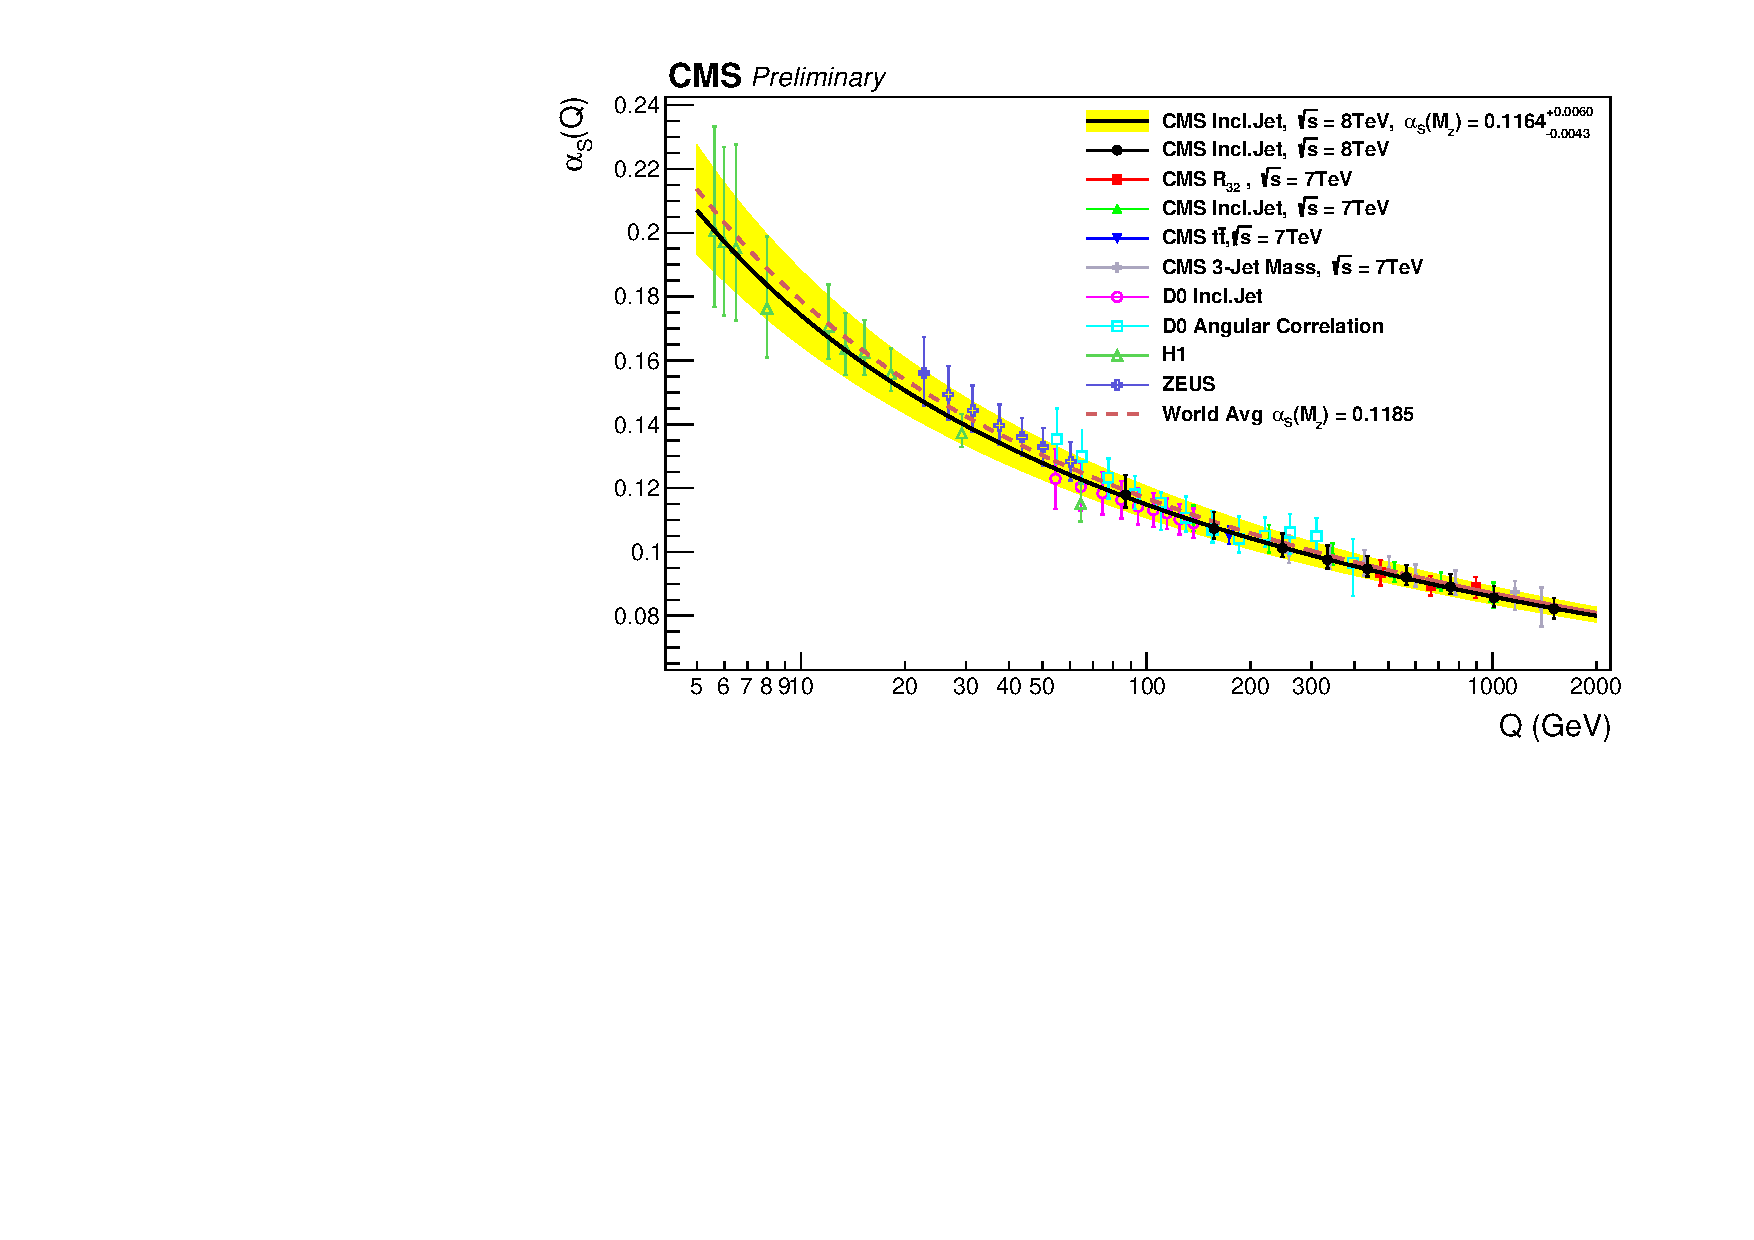
\includegraphics[width=0.9\textwidth]{Figure4.pdf}
 \caption{The running \asq as a function of the scale $Q$ is shown, as
   obtained by using the CT10 NLO PDF set. The solid line and the
   uncertainty band are obtained by evolving the extracted \alpsmz
   values by using the 2-loop 5-flavour renormalization group
   equations. The dashed line represents the evolution of the world
   average value. The black dots in the figure show the numbers
   obtained from the $\sqrt{s}=8$\TeV inclusive jet
   measurement. %Results from other CMS%~\cite{R32, CMSTTBar, CMS-PAS-SMP-12-027}
   %, D0%~\cite{D0Alpha1, D0Alpha2}
   %, H1%~\cite{H1Alpha1, H1Alpha2}
   %, and ZEUS%~\cite{ZEUSAlpha}
   %measurements are superimposed.
 }
\label{fig:AlphasRun}
\end{figure*}

The ATLAS Collaboration has recently measured the strong coupling constant using the transverse energy-energy
correlation (TEEC) function and its associated azimuthal asymmetry in multi-jet events at a
centre-of-mass energy of 7 \TeV~\cite{ATLAS:2015yaa}. The average transverse momentum of the two leading jets is
required to be larger than 250 GeV. The TEEC distribution is obtained from the $\cos\Delta\phi_{ij}$ between any pair of
jets $i$ and $j$, weighted by $$w_{ij} = \frac{E_{Ti}E_{Tj}}{(\sum_k E_{Tk})^2} \, ,$$ where $E_T$ is the jet transverse
energy and the sum runs over all the jets in the event. With respect to other observables the TEEC are less sensitive to the jet energy scale and resolution,
and to PU. The measured TEEC distribution is shown in Figure~\ref{fig:TEEC}, after unfolding for the effect of
the detector. In the same the result of a fit to pQCD NLO calculations from \NLOJETPP including NP
corrections is also shown. 
\begin{figure*}[hbpt]
  \centering
  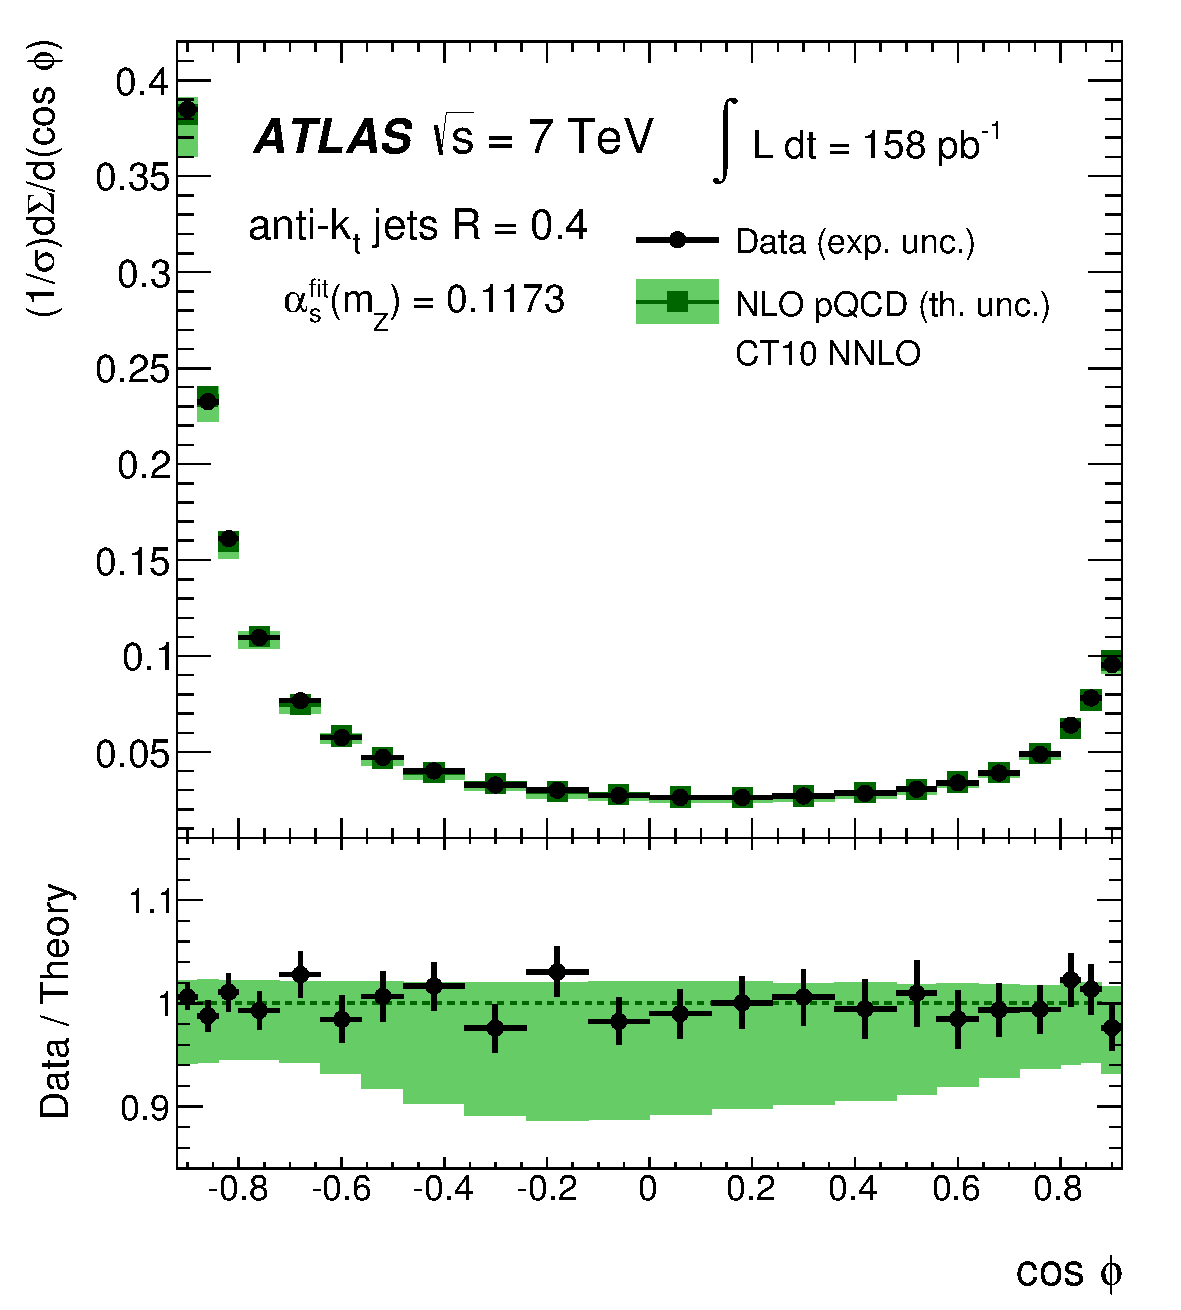
\includegraphics[width=0.6\textwidth]{Figure5.pdf}
  \caption{The unfolded distributions for transverse energy-energy correlation compared with the results of a fit to
    pQCD NLO calculations including NP corrections. The green shaded band indicates the uncertainty on the
    theoretical predictions, which includes the sum in quadrature of uncertainties associated with scale, \as, PDF and
    NP corrections.}
  \label{fig:TEEC}
\end{figure*}
The measured value of \alpsmz is 
$$ \alpsmz  = 0.1173 \pm 0.0010 \mathrm{(exp.)} ^{+0.0063}_{-0.0020} \mathrm{(scale)} \pm 0.0017 \mathrm{(PDF)} \pm
0.0002 \mathrm{(NP)} \, $$
and it is also in agreement with the world average. This value has been obtained with the CT10 NLO PDF set, which has
the largest PDF uncertainty, covering the variations with different PDF sets.


The ATLAS Collaboration recently studied 4-jets events at 8 \TeV\cite{Aad:2015nda}, exploring many variables sensitive to the topology and the
different energy scales of the event. These observables have been compared to predictions from several MC
generators and from fixed-order NLO calculations. The maximum rapidity difference among a jet pair, $\Delta
y_{2j}^{max}$, shown in Figure~\ref{fig:4jet}, is one of the variables where some discrepancies are observed. 
The NLO predictions, \BLACKHAT/\SHERPA~\cite{Berger:2008sj,Bern:2011ep} and
\NJET/\SHERPA~\cite{Badger:2012pg,Badger:2012pf}, are almost always compatible with the data within their 
theoretical uncertainties. The \HEJ~\cite{Andersen:2009nu,Andersen:2011hs} all-orders calculation and the multi-leg calculation with up to four partons in the
matrix element (ME) generated by \MADGRAPH~\cite{Alwall:2014hca} and matched to the \PYTHIAS~\cite{Sjostrand:2006za} PS also provides a good description of
the data. The $2\ \to 2$ MC generators \PYTHIAE and \HERWIGpp~\cite{Bahr:2008pv}
 describe the data relatively poorly. These results show therefore 
the importance of the more sophisticated calculations in a variety of scenarios. 

\begin{figure*}[hbpt]
  \centering
  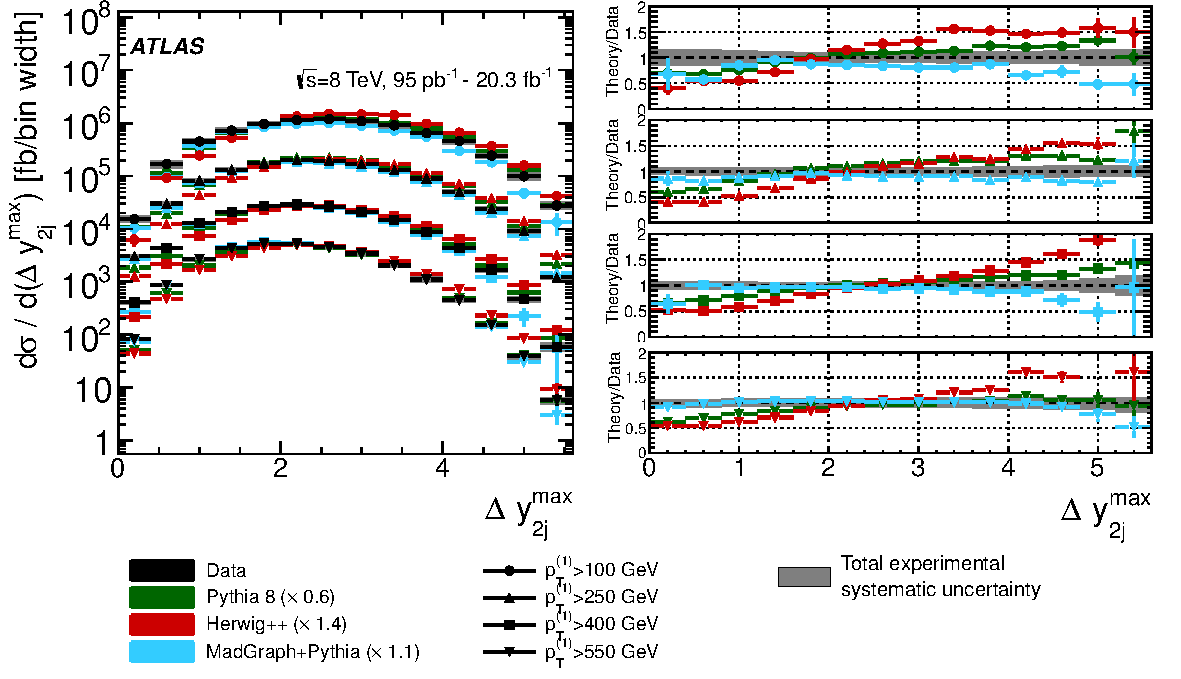
\includegraphics[width=0.9\textwidth]{Figure6a.pdf}\\
  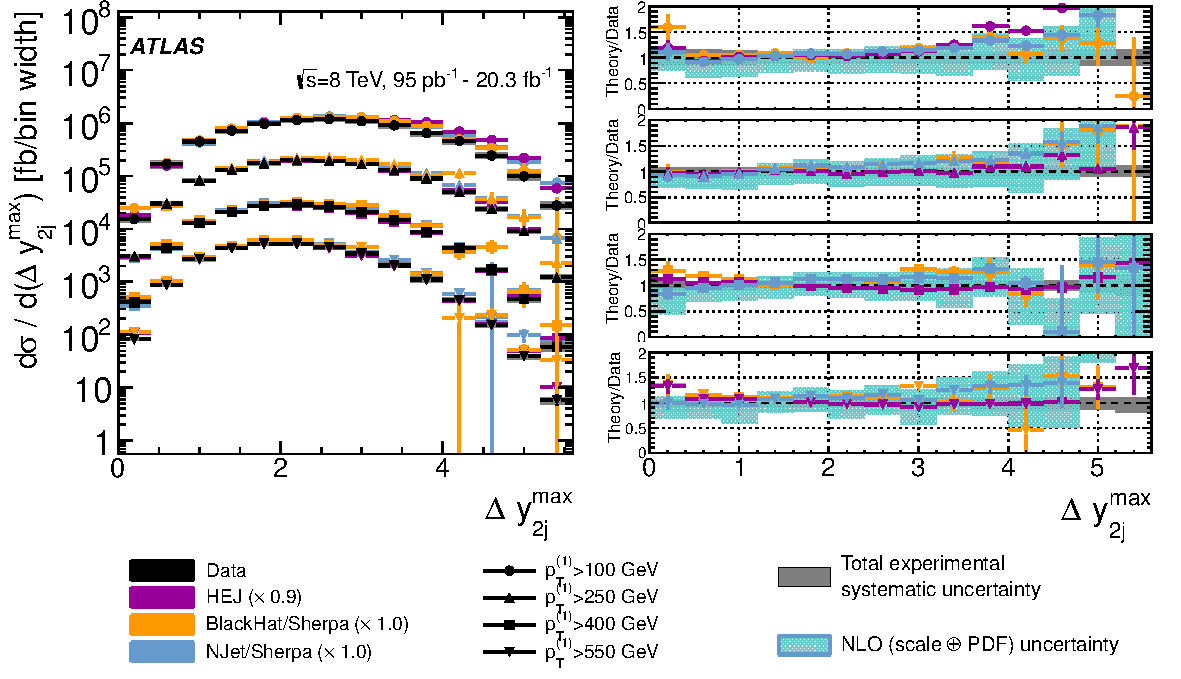
\includegraphics[width=0.9\textwidth]{Figure6b.pdf}
  \caption{Unfolded four-jet differential cross section as a function of $\Delta y_{2j}^{max}$, compared to different
    predictions: \PYTHIAE, \HERWIGpp and \MADGRAPH+PYTHIAS (top), and HEJ, \NJET/\SHERPA and \BLACKHAT/\SHERPA (bottom). The MC
    and \HEJ predictions are multiplied by the factors indicated in the legend in order to be normalized to the events observed in the data. The left 
    panel shows the full spectra and the right panel the ratios of the different predictions to the data. The solid band represents the total experimental systematic
    uncertainty centred at one. The patterned band represents the NLO scale and PDF uncertainties calculated from
     \NJET/\SHERPA. The scale uncertainties for \HEJ (not drawn) are typically
    +50\%-30\%. The ratio curves are formed by the central values and vertical uncertainty lines resulting from the
    propagation of the statistical uncertainties of the predictions and those of the unfolded data spectrum.} 
  \label{fig:4jet}
\end{figure*}

The CMS Collaboration has also recently published new studies of the properties of multi-jets events at 7\TeV~\cite{Khachatryan:2016udy, Khachatryan:2015xwa} and
8~\TeV~\cite{Khachatryan:2016hkr}. In Figure~\ref{fig:dijet} the azimuthal decorrelation $\dphi$ between the two jets with the largest transverse momenta at
8\TeV is presented for seven regions of leading jet transverse momentum \ptmax up to 2.2\TeV. The dijet azimuthal decorrelation is caused by
the radiation of additional jets and probes the dynamics of multi-jet production. The results are compared to calculations in
pQCD calculations from \NLOJETPP with the CT10 NLO PDF set for 3-jet production with up to four outgoing partons.
These fixed-order calculations provide NLO predictions for the range of
$2\pi/3 \leq \dphi < \pi$, corresponding to a final state with at least 3 jets, and LO predictions for $\pi/2 \leq \dphi <
2\pi/3$, where at least 4-jets must be present. The predictions are normalized separately in these two region and
describe the data well over several order of magnitude, though they increasingly deviate from data for lower values of
\dphi, especially at low \ptmax. 

\begin{figure}[hbtp]
  \centering
  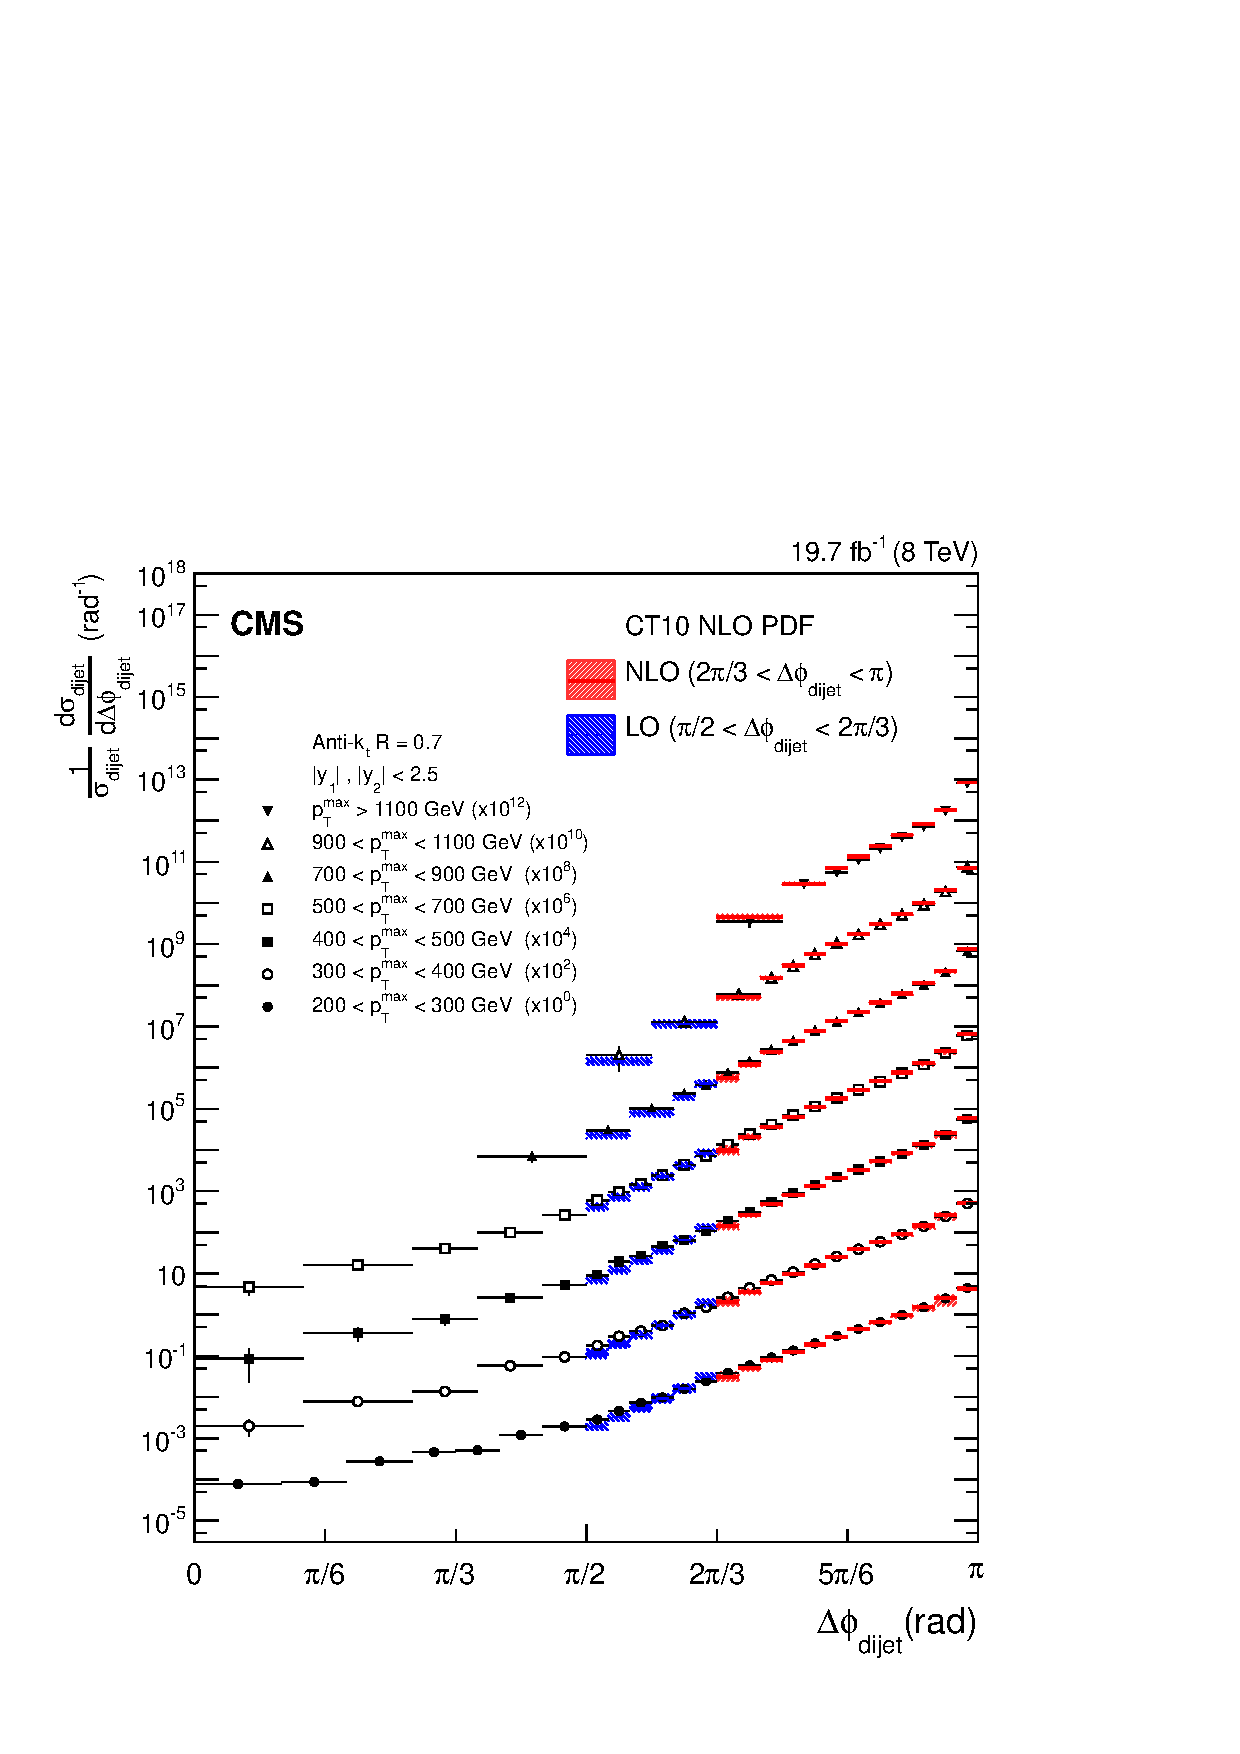
\includegraphics[width=0.6\textwidth]{Figure7a.pdf}
  \caption{Normalized dijet cross section differential in \dphi for
    seven \ptmax regions, scaled by multiplicative factors for
    presentation purposes.  The error bars on the data points include
    statistical and systematic uncertainties. Overlaid on the data
    (points) are predictions from LO (dashed line; $\pi/2 \leq
    \dphi < 2\pi/3$) and NLO (solid line; $2\pi/3 \leq \dphi \leq
    \pi$) calculations using the CT10 NLO PDF set. 
    % and excluding the bin at $\dphi=\pi$.
%    The PDF, \as, and scale uncertainties are
%    added in quadrature to give the total theoretical uncertainty, which
%    is indicated by the downwards-diagonally (LO) and
%    upwards-diagonally (NLO) hatched regions around the theory lines.
}
  \label{fig:dijet}
\end{figure}

In Figure~\ref{fig:dijet_ratios_MC_data} the ratio of several MC generators predictions to
the the data is shown. Similar conclusions as for the 4-jets analysis performed by ATLAS can be drawn. Event generators with only two outgoing
partons at matrix-element fail to describe the measurement. This apply also to \POWHEG that has NLO 
QCD corrections matched to the \PYTHIAE PS. In the case of \MADGRAPH+\PYTHIAS from two to four outgoing partons are
provided by the ME calculations and are matched to the PS, providing a very good description of the data down to very
low \dphi values.  

\begin{figure*}[hbtp]
  \centering
  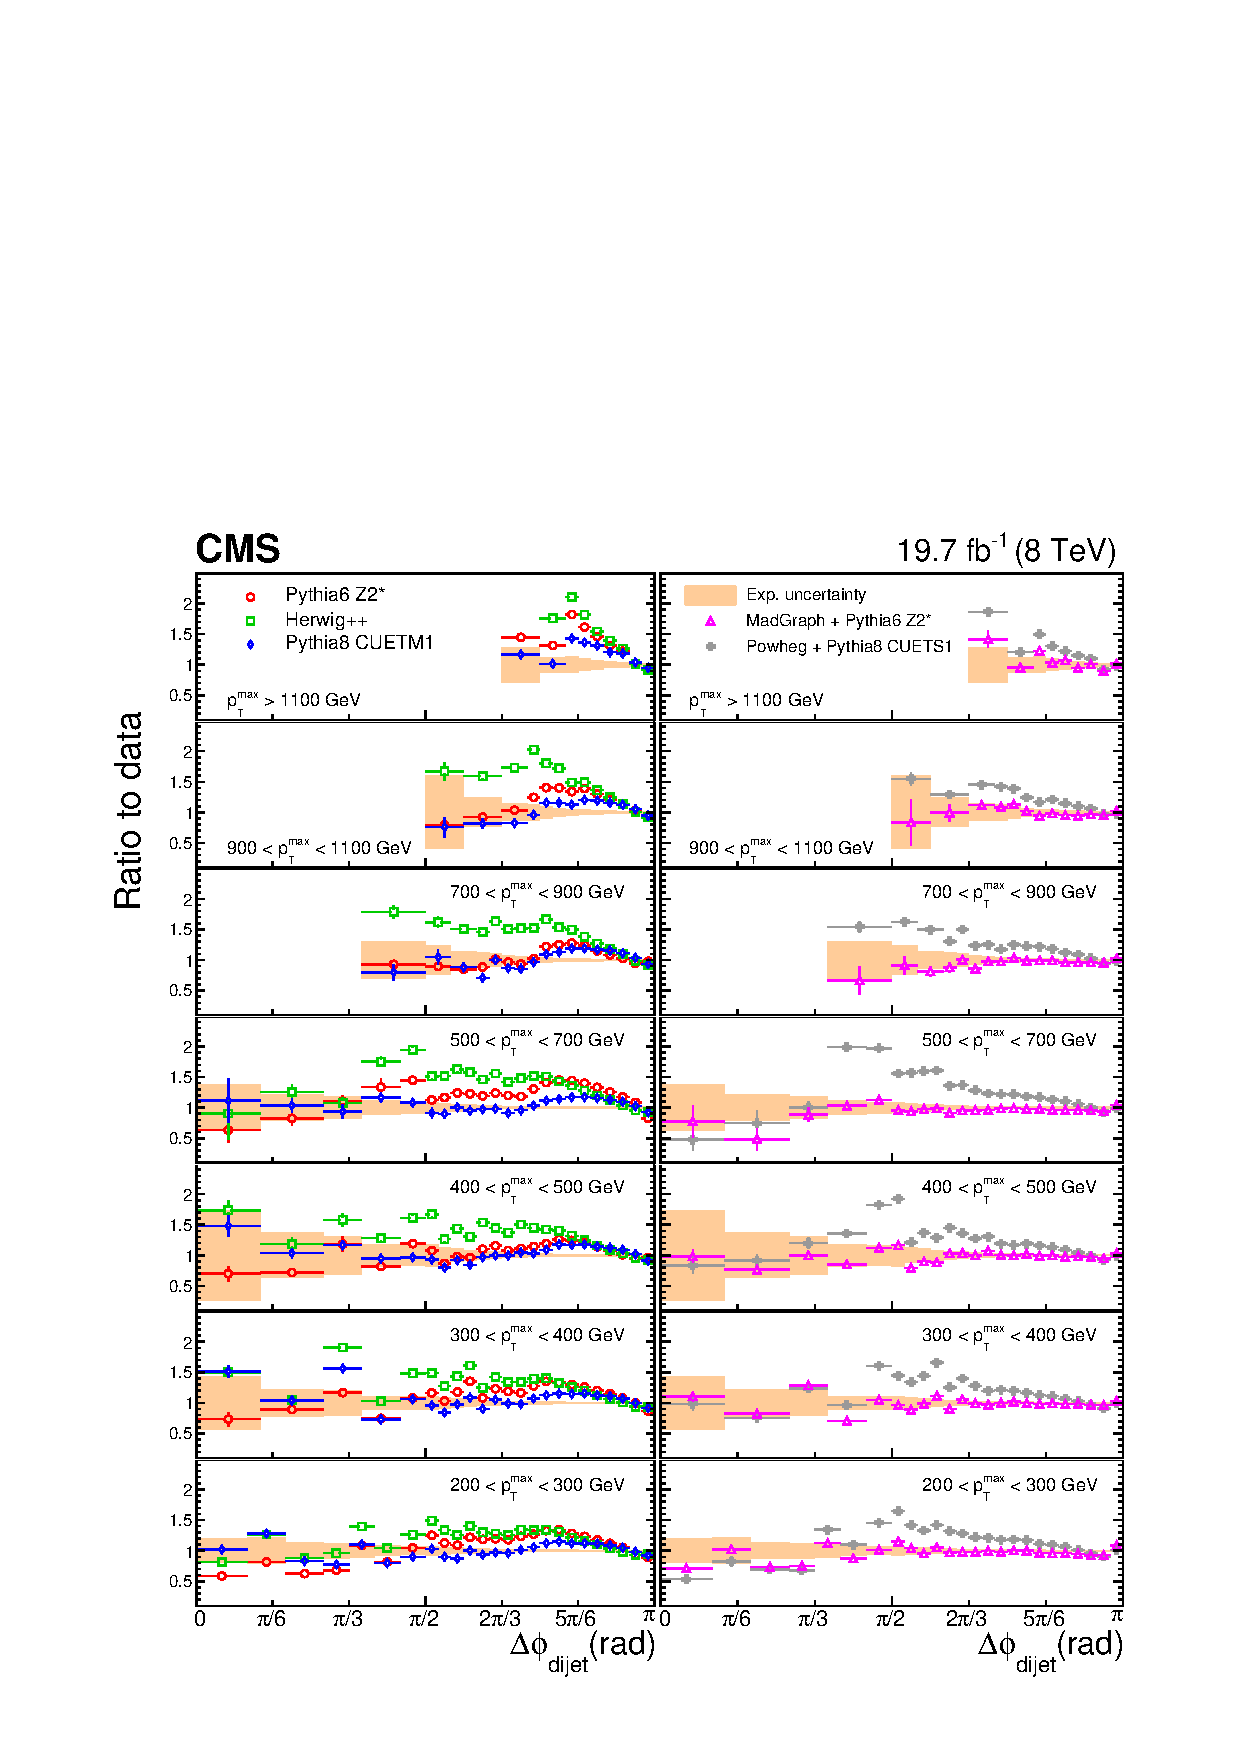
\includegraphics[width=0.6\textwidth]{Figure8.pdf}
  \caption{Ratios of \PYTHIAS, \HERWIGpp, \PYTHIAE, \MADGRAPH + \PYTHIAS, and
    \POWHEG + \PYTHIAE predictions to the normalized dijet cross
    section differential in \dphi, for all \ptmax regions.
    The solid band indicates the total experimental uncertainty and
    the error bars on the MC points represent the statistical
    uncertainties of the simulated data.}
  \label{fig:dijet_ratios_MC_data}
\end{figure*}

Jets are not only a probe for pQCD or other high transverse momentum processes. They are also interesting for their
properties, which depends mostly on quark fragmentation and hadronisation. An example of this kind of studies is the
measurement of charged-particle multiplicity $<n_\mathrm{charge}>$ in jets performed by ATLAS on the 8~\TeV data sample~\cite{Aad:2016oit}.
The multiplicity is measured including charged tracks with $\pt > 0.5$, 2 or 5~\GeV, for jets with $\pt > 50$~\GeV and up to
$1.5$~\TeV. Results are compared to \HERWIGpp, \PYTHIAS and \PYTHIAE with different underlying event tunings, showing
that the description of data improves for the most recent tunes. 
The charged multiplicity is important to discriminate between quarks- and gluon-initiated jets, being larger in the case
of a gluon jet. For this reason after unfolding the results for detector effects, the  $<n_\mathrm{charge}>$ is
extracted separately for quark and gluon jets as a function of the jet transverse momentum. Results are shown in
Figure~\ref{fig:chargemult} and confirm that this number is larger for gluon jets as expected, with a dependence on the jet transverse
momentum.

\begin{figure*}[hbtp]
  \centering
  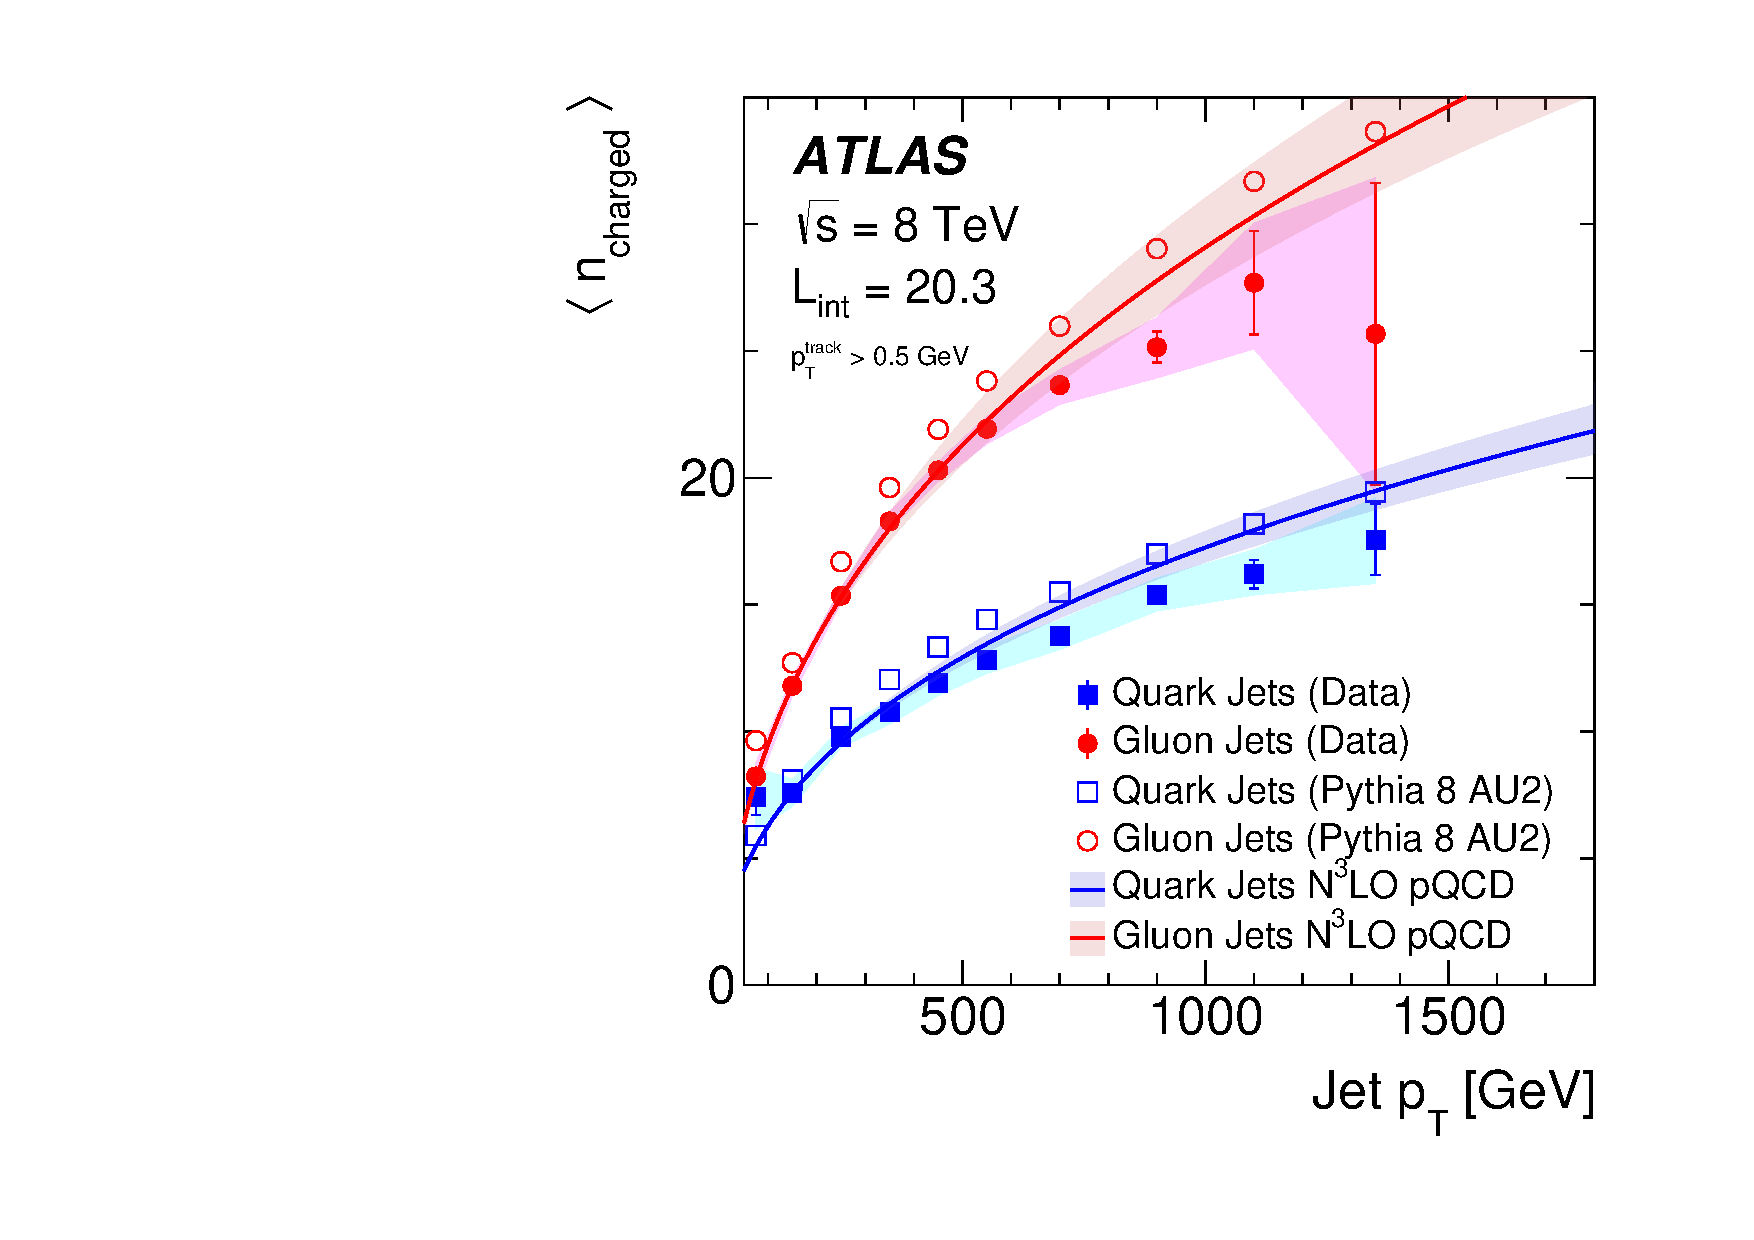
\includegraphics[width=0.6\textwidth]{Figure9.pdf}
  \caption{Jet \pt dependence of charged-particle multiplicity, for tracks $\pt > 0.5$~\GeV, for quark- and
    gluon-initiated jets.}
  \label{fig:chargemult}
\end{figure*}

The jet charge is another observable recently measured using 8~\TeV data by ATLAS~\cite{Aad:2015cua} and
CMS~\cite{CMS:2016yuu}. The jet charge is the \pt weighted sum of the charge of the particles in a
jet. It is defined as 
%%%
\begin{equation} \label{Omdef}
Q^\kappa = \frac{1}{(\pt)^\kappa} \sum_{i} Q_i (\pt^i)^\kappa
\end{equation}
%%%
where the sum is over all particles i in the jet with \pt $>$ 1 \GeV, $Q_i$ is the charge of the particle, $\pt^i$ is
the particle transverse momentum, and $\kappa$ is a free parameter. The charge of the leading jet in dijets events is
considered and different values of $\kappa$ are used: 0.3, 0.5, 0.7 by ATLAS; 0.3, 0.6, 1.0 by CMS. In addition ATLAS
measured also the standard deviation, while CMS used alternative definitions of the jet charge based on transverse and
longitudinal momentum of the particles with respect to the jet axis. ATLAS results are shown in
Figure~\ref{fig:jetcharge} compared to MC predictions obtained using the CT10 NLO or the
CTEQ6L1~\cite{Pumplin:2002vw}. The LO prediction agree with data within 5\%, while the NLO predictions are generally
about 10\% below the data. There does not seem to be an effect from the POWHEG NLO matrix element.   
This observation is consistent with the expectation that the PDF and (nearly collinear) fragmentation
are responsible for the jet charge distributions.    

\begin{figure*}[hbtp]
  \centering
  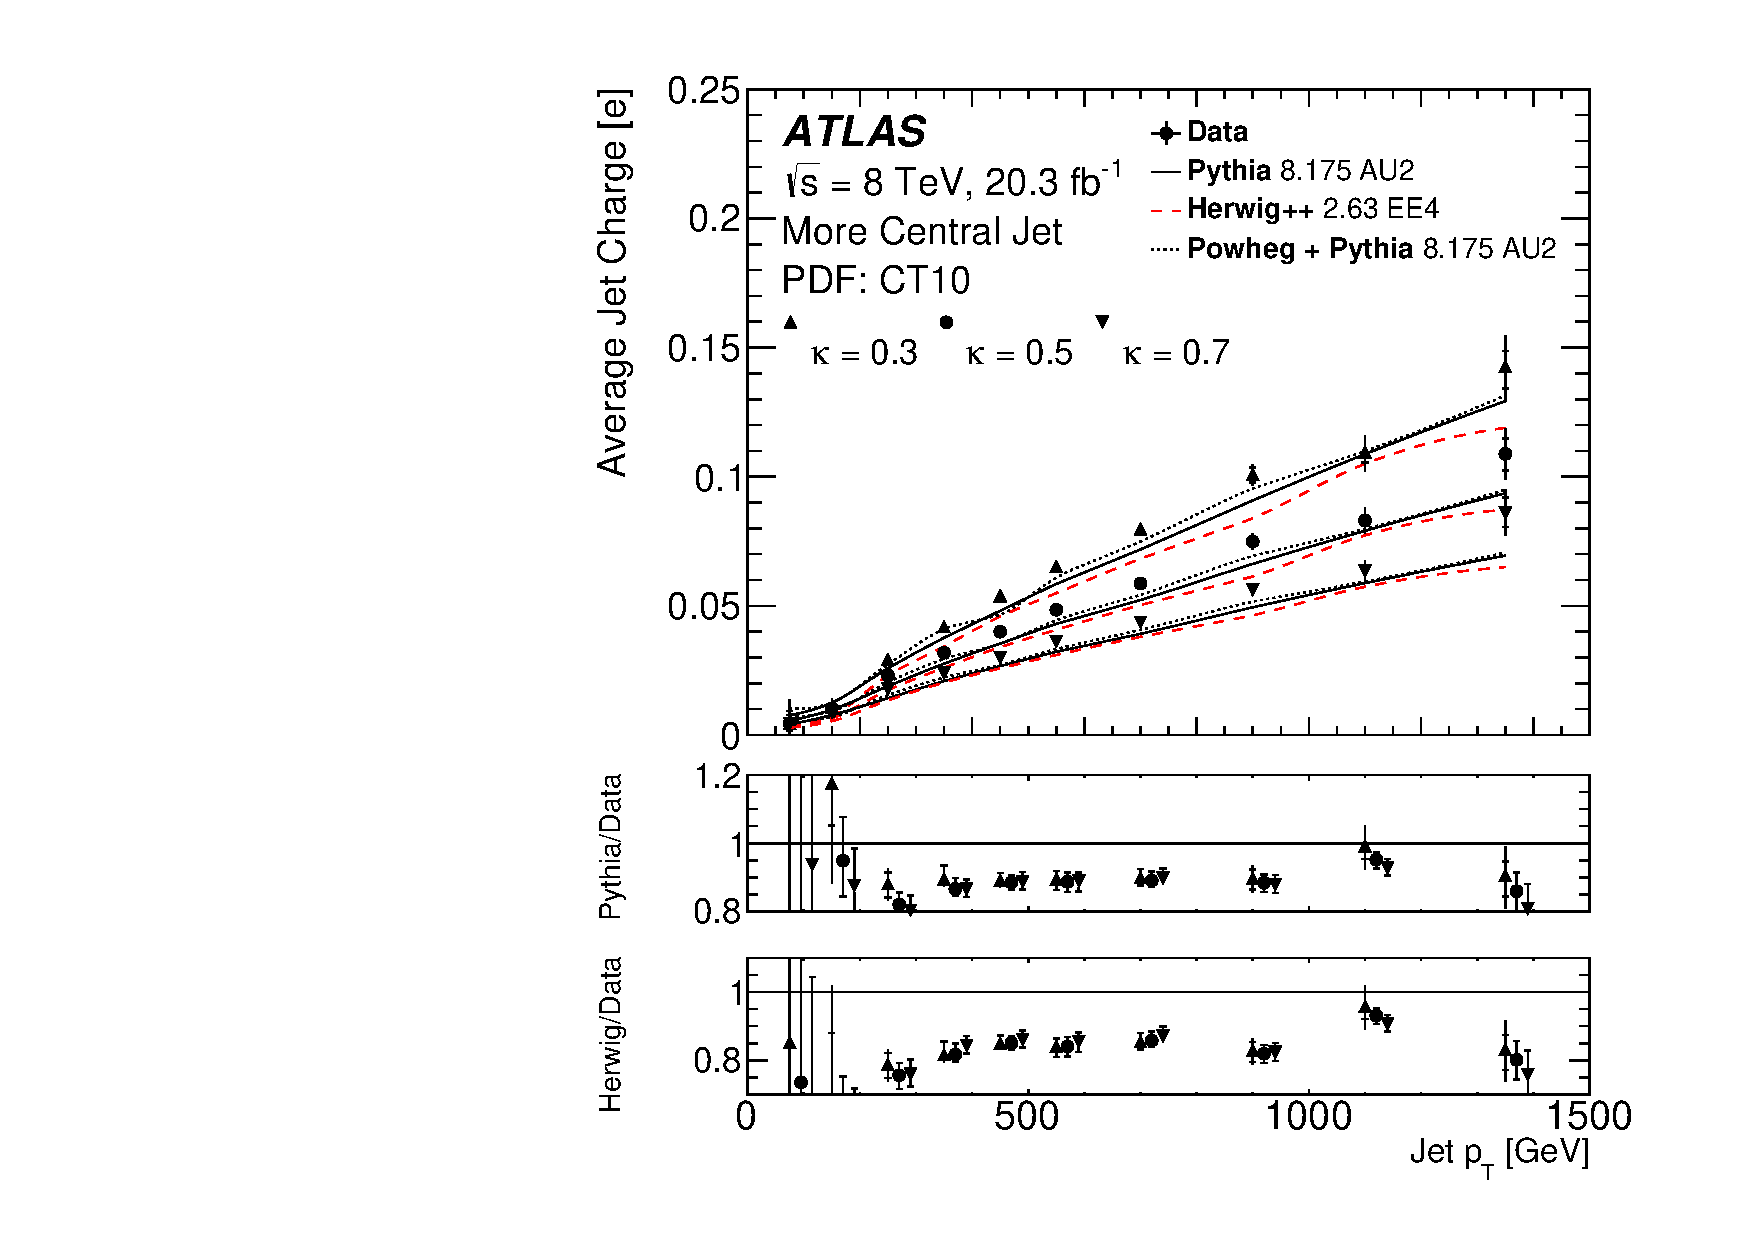
\includegraphics[width=0.48\textwidth]{Figure10a.pdf}
  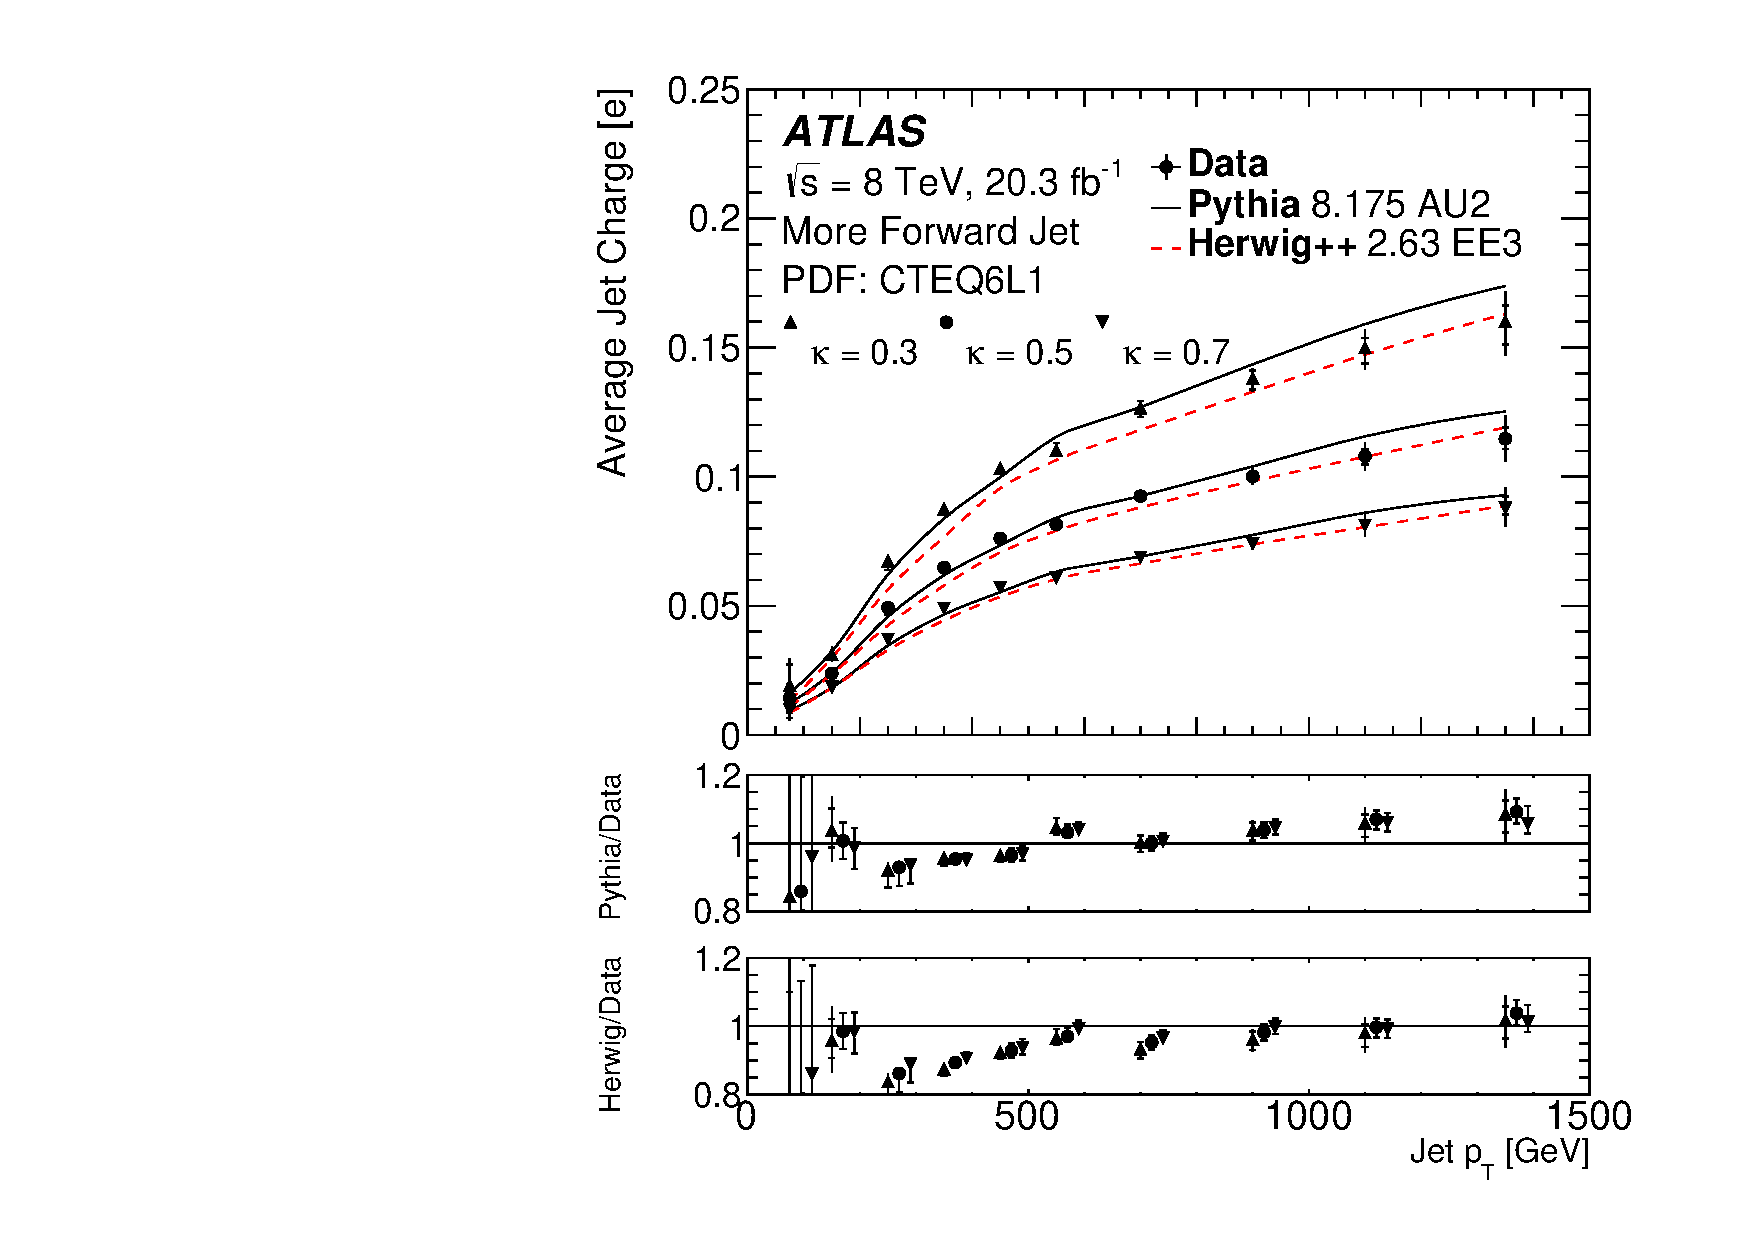
\includegraphics[width=0.48\textwidth]{Figure10b.pdf}
  \caption{The measured average of the jet charge distribution in units of the positron charge as a function of the jet
    \pt for $\kappa=$0.3, 0.5, and 0.7 for the more central jet using CT10 (left) or CTEQ6L1 (right) as the PDF set. The crossed lines in the
    bars on the data indicate the systematic uncertainty and the full extent of the bars is the sum in quadrature of the
    statistical and systematic uncertainties. } 
  \label{fig:jetcharge}
\end{figure*}


\section{Photon Physics}

Prompt photons are those produced in the hard process, mainly through the LO process $qg \to q\gamma$, and can therefore
be used to study the gluon PDF. In addition, they are an important background to many interesting channel, e.g. Higgs
decays into diphotons, therefore their production needs to be precisely measured.  
The dominant background to prompt photon production are photons originating from light neutral mesons decay ($\pi^0,
\eta$). Furthermore, inclusive prompt photon production is made up of direct and fragmentation photons: direct photons
are produced in the hard process, whereas fragmentation photons are generated in the parton fragmentation process. The
photon selection is designed to suppress the background from hadron decays, but also to reduce the fragmentation
contribution, which is a less understood non-perturbative process, by applying an isolation requirement. 

The photon recontruction and identification starts from a cluster of energy deposits in the electromagnetic calorimeter
(ECAL), supplemented by the informations in the tracker detector. If there are no tracks pointing to the cluster it is an
unconverted photon candidate, while if there are two tracks coming from a conversion vertex or one track with no hits in
the pixel detector it is a converted photon. Both candidates are kept for the following analysis, which is then tuned
depending on the type. 

In ATLAS photons are identified with a likelihood based on nine variables related to the lateral and longitudinal
development of the shower in the LAr sampling ECAL~\cite{ATLAS:2012ana}. In CMS the photon identification is
based on the shape of the electromagnetic shower in the lead tungstate crystal ECAL~\cite{Chatrchyan:2013dga}.
Both experiments apply in addition an isolation requirement to further remove the background and the fragmentation
photons as explained above. The identification with the shower shape and the isolation are partially uncorrelated and
it is possible to extract from data the purity of the selected photon sample from the distribution in this two variables. 

ATLAS recently published the inclusive prompt photon cross-section at 8~\TeV~\cite{Aad:2016xcr}. The measurement is
performed for photons with an energy between 25 \GeV and 1.5 \TeV, and for a pseudorapidity of up to $\eta = 2.37$. 
Results are shown in Figure~\ref{fig:photon} together with NLO predictions from \JETPHOX~\cite{Catani:2002ny}. 
\begin{figure}
\begin{center}
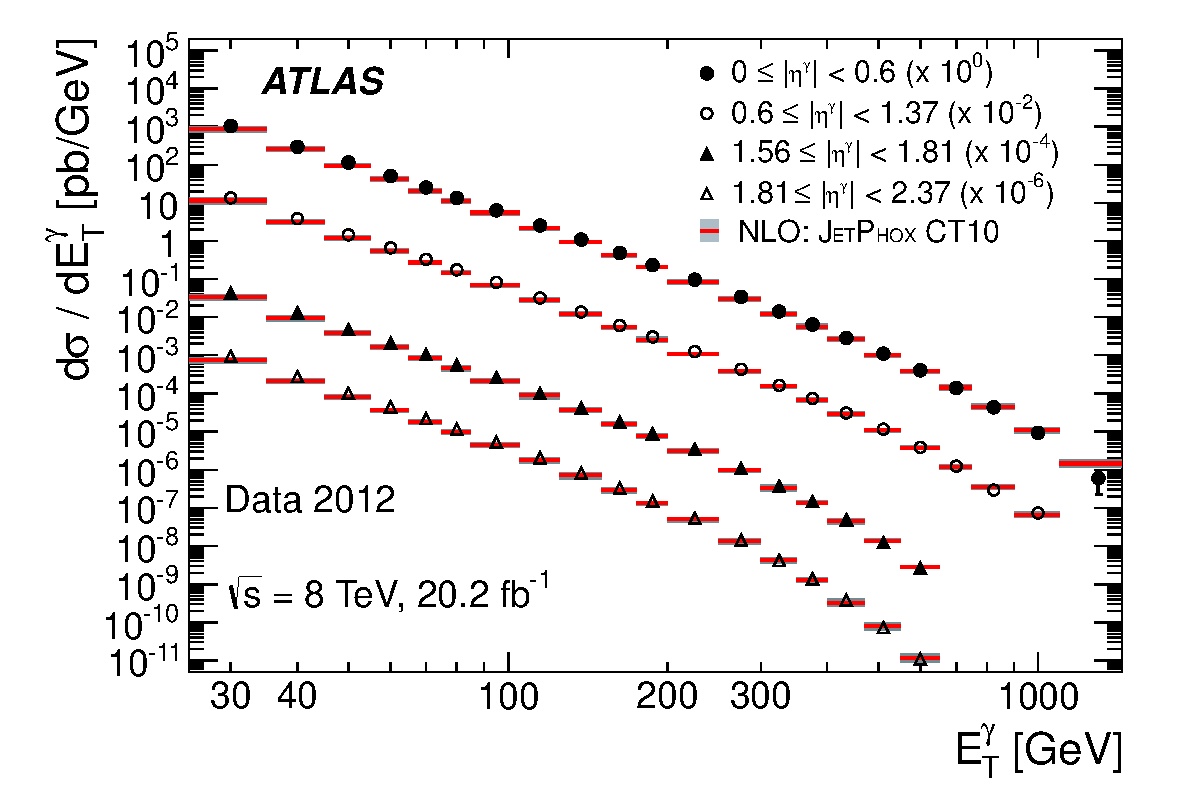
\includegraphics[width=0.6\textwidth]{Figure11.pdf} 
\caption{Differential cross sections of prompt photons in 8 \TeV data, with \JETPHOX predictions superimposed. The
  distributions are scaled by the specified factors to separate them visually. }  
\label{fig:photon}
\end{center}
\end{figure}
Figure~\ref{fig:photon_MC} shows the ratio of the theory predictions to the data: in addition to \JETPHOX, the MC programs
\PYTHIA and \SHERPA are shown. Predictions from \JETPHOX with CT10 PDF set are ~20\% lower than the data, though compatible within the
uncertainty from the scale, \as, PDF, hadronisation and underline event. Results from \SHERPA, with CT10 PDF, and \PYTHIA, with
CTEQ6L1 PDF, show some significant deviations from the data: \SHERPA is better for central photons, while
\PYTHIA is in good agreement with data for high $|\eta|$. In the case of \SHERPA up to four partons can be present in the
final state and the parton shower treats coherently gluon and photon emissions. That means that it is not possible to
distinguish between direct and fragmentation photons. \PYTHIA instead does the LO direct production in the ME and the
fragmentation in the PS. As already noted, none of the two approaches is able to describe the data in the whole energy
and pseudorapidity range.
\begin{figure}
\begin{center}
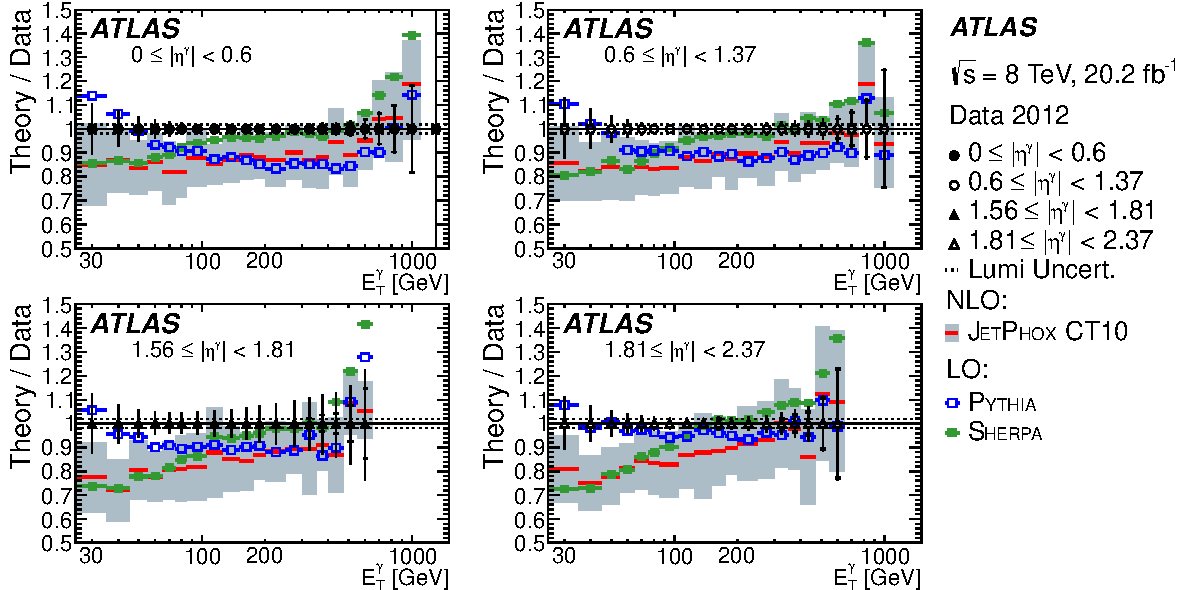
\includegraphics[width=0.9\textwidth]{Figure12.pdf} 
\caption{Ratio of theory (PYTHIA, SHERPA and \JETPHOX) to data for the differential prompt photon cross sections. The
  statistical component of the uncertainty in the data is indicated by the horizontal 
  tick marks whereas the whole error bar corresponds to the combined statistical and systematic uncertainty. The
  additional systematic uncertainty arising from the uncertainty in the integrated luminosity is displayed separately as
  a dotted line. The total uncertainty on \JETPHOX calculations is displayed as a band. }  
\label{fig:photon_MC}
\end{center}
\end{figure}

The CMS experiment has measured the differential cross sections for the production of a photon pair in association with
jets at $\sqrt{s}=7$~TeV~\cite{CMS:2015hha}. The fraction of prompt diphoton events in data is extracted from a template fit to the photon
isolation distribution. The signal template has been obtained from the data itself with the ``random cone''
technique, where the isolation energy in a region separated from the photon. Several differential observables are
studied with inclusive 1-jet and 2-jet selections and results are compared to LO and NLO QCD theoretical predictions
from \SHERPA, \AMCATNLO~\cite{Alwall:2014hca}, and \GOSAM~\cite{Gehrmann:2013aga} event generators. As an example, the
angular correlations between the leading jet and the photons are shown in Figure~\ref{fig:diphot}. 
\begin{figure}
\begin{center}
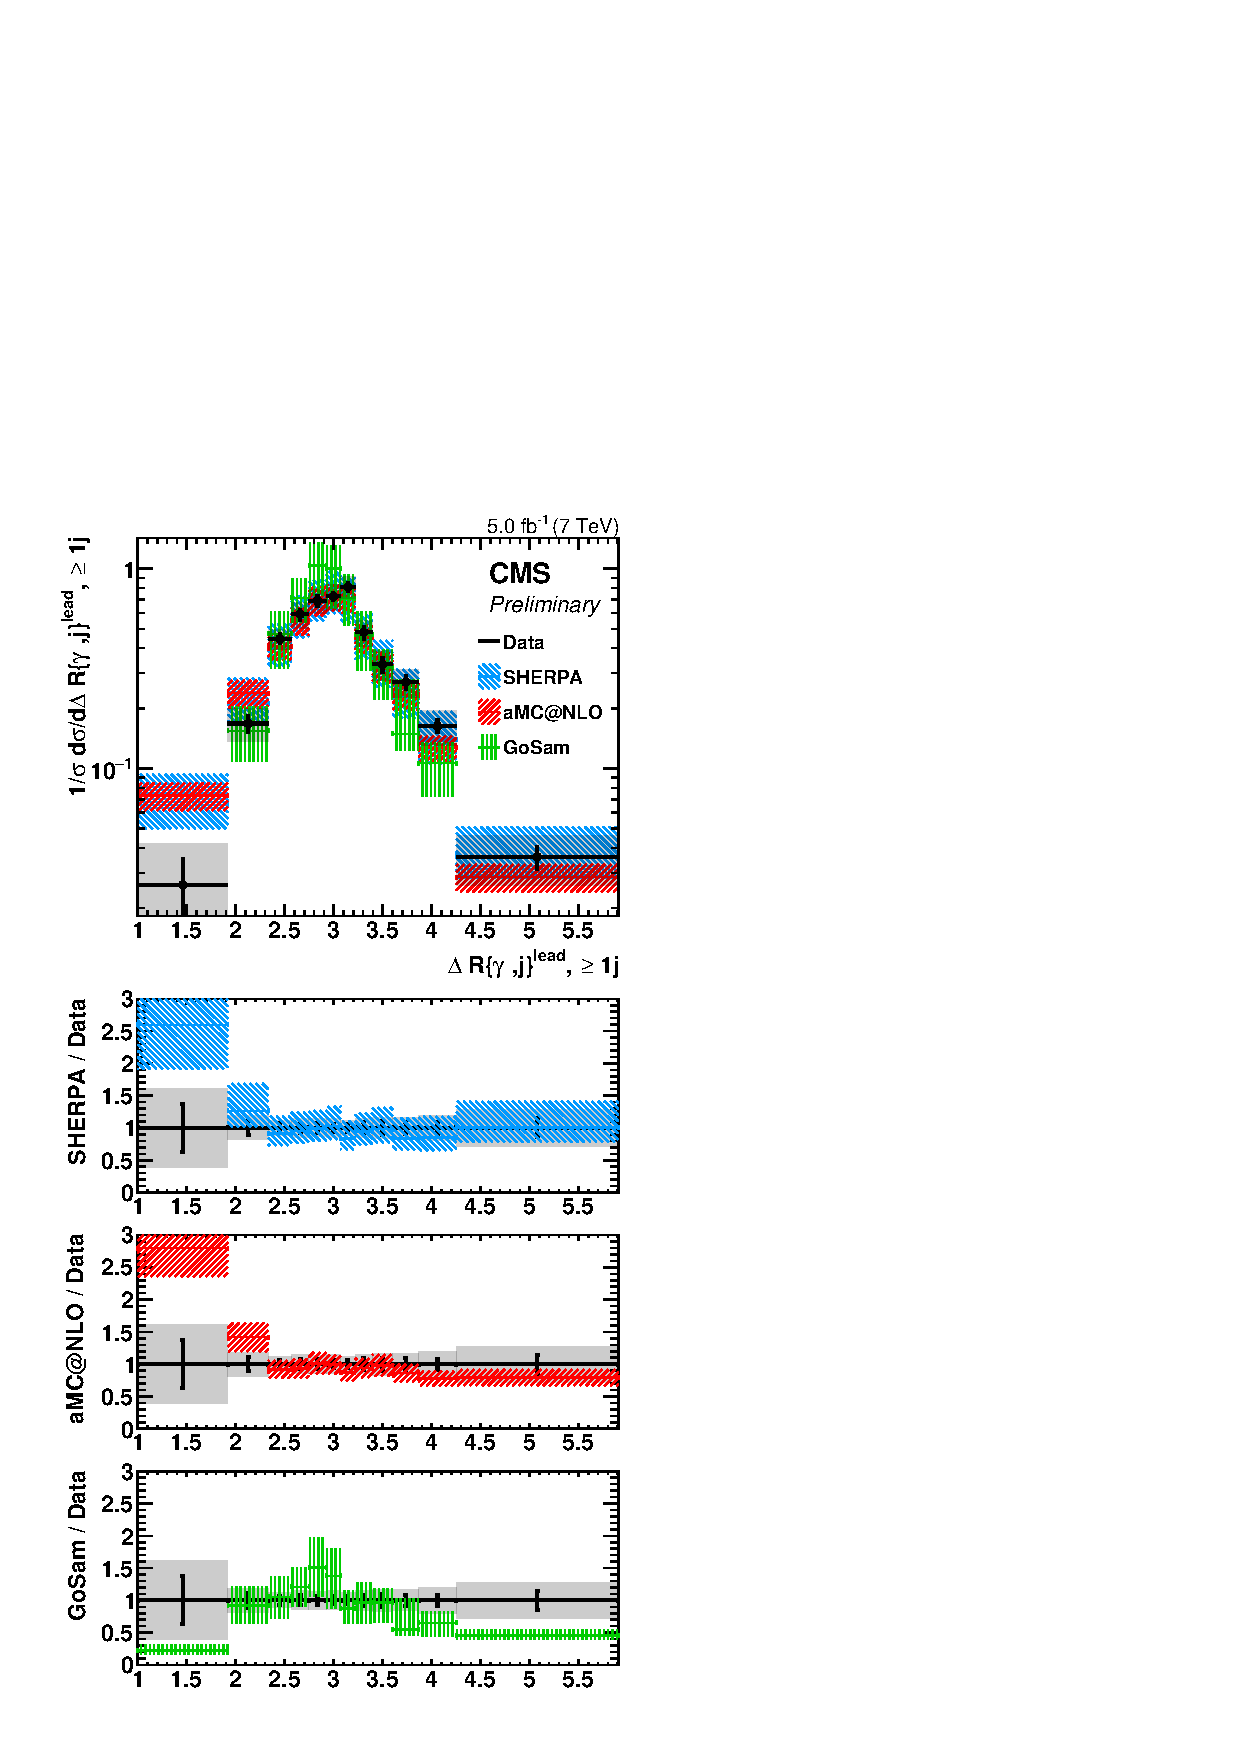
\includegraphics[width=0.48\textwidth]{Figure13a.pdf}
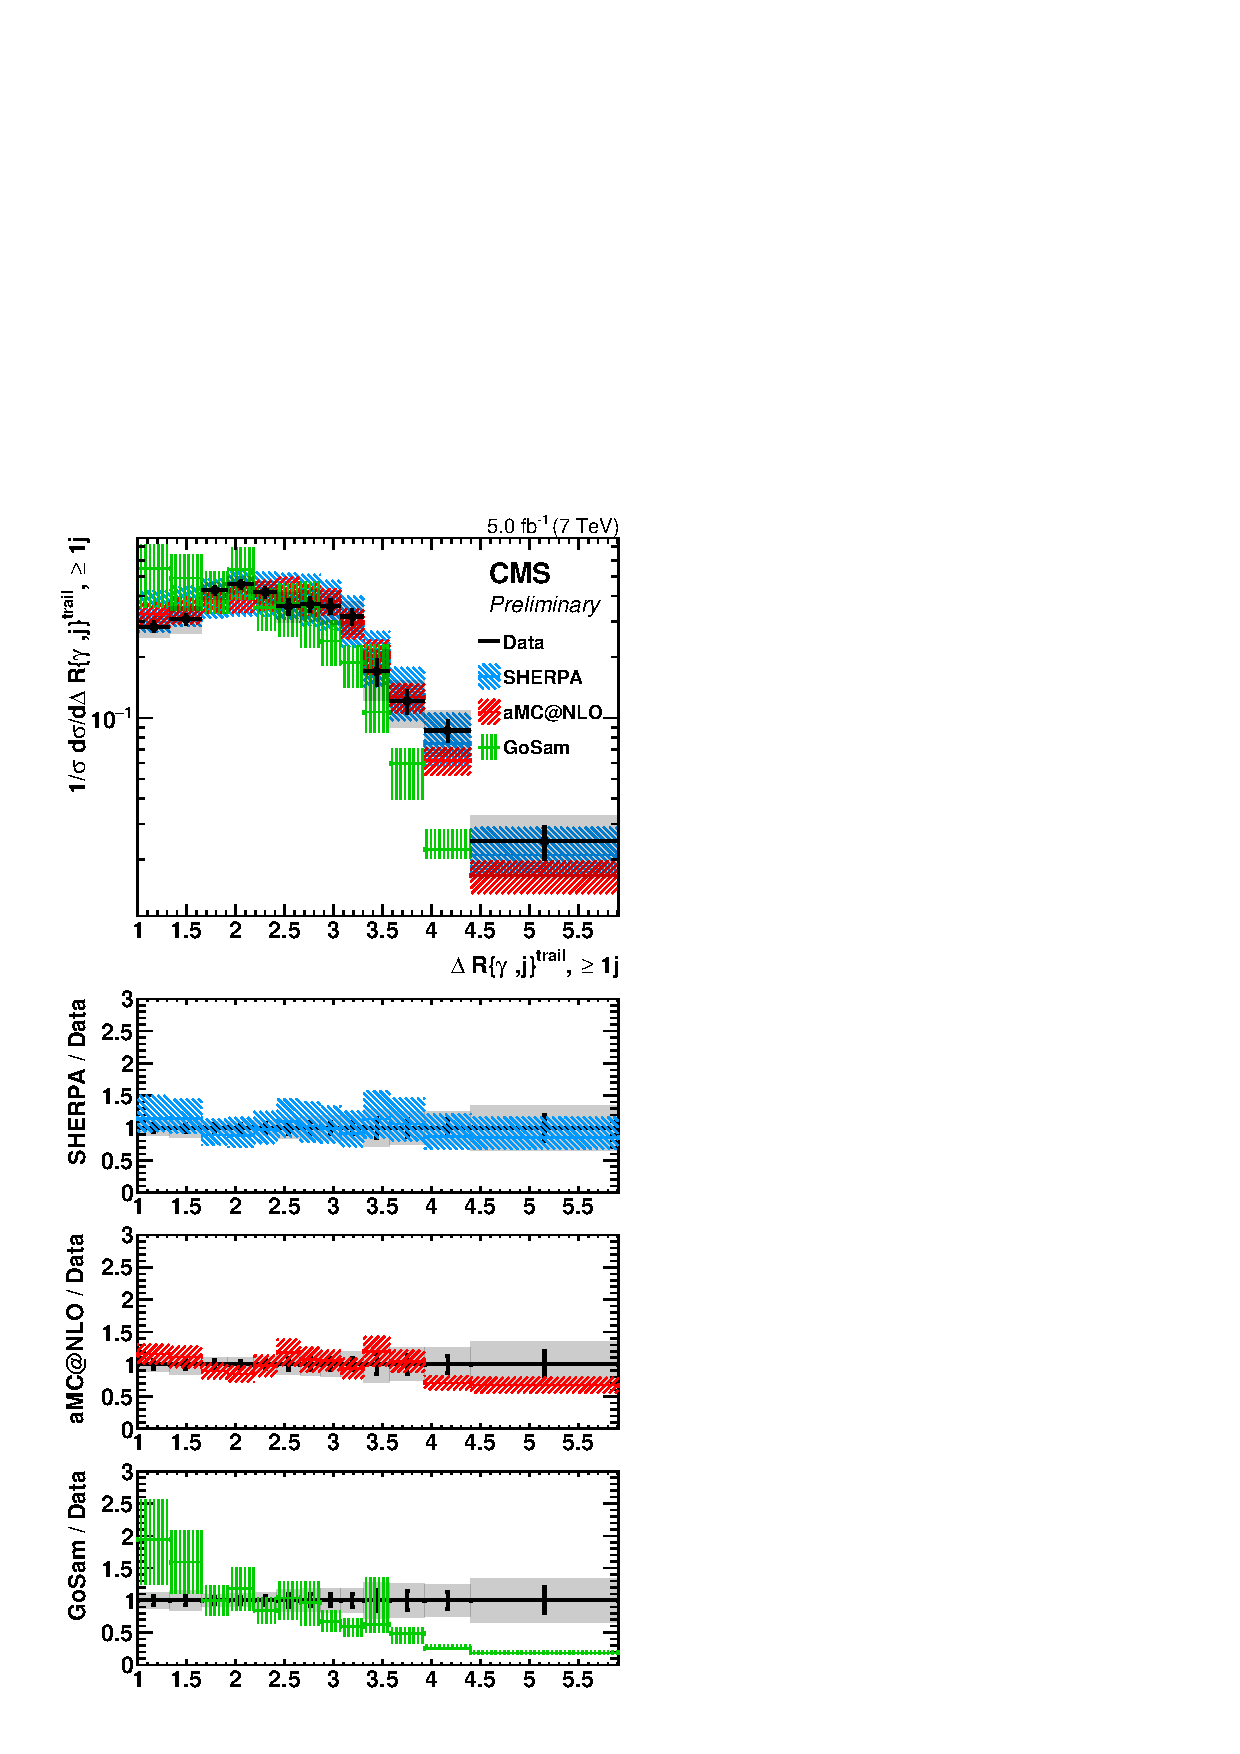
\includegraphics[width=0.48\textwidth]{Figure13b.pdf}
\caption{Differential cross section as a function of the $\Delta R$ separation between the leading jet and the leading (left) or subleading (right) photon. All distributions are normalized to unitary area.}
\label{fig:diphot}
\end{center}
\end{figure}
The \SHERPA and
\AMCATNLO predictions agree with the data for a large set of differential 
observables. The parton-level \GOSAM prediction also describes the data well except for the angular correlations between
photons and jets, where discrepancies are observed.

Finally, the ratio of the associated production of a $\mathrm{Z}/\gamma^*$ or a $\gamma$ with one or more jets has been recently measured in
proton-proton collisions at 8 TeV center-of-mass energy by CMS~\cite{Khachatryan:2015ira}.
In the limit of high transverse momentum of the vector boson the effects due to the mass of the Z
boson are small, and the cross section ratio of Z+jets to $\gamma$+jets is expected to become constant. 
Figure~\ref{zgrNLO} compare the data to for events with a vector boson and at least one
jet to fixed-order predictions from \SHERPA+\OPENLOOPS including both QCD and EW NLO corrections~\cite{Kallweit:2014xda,Kallweit:2015dum}. 
\begin{figure}
\begin{center}
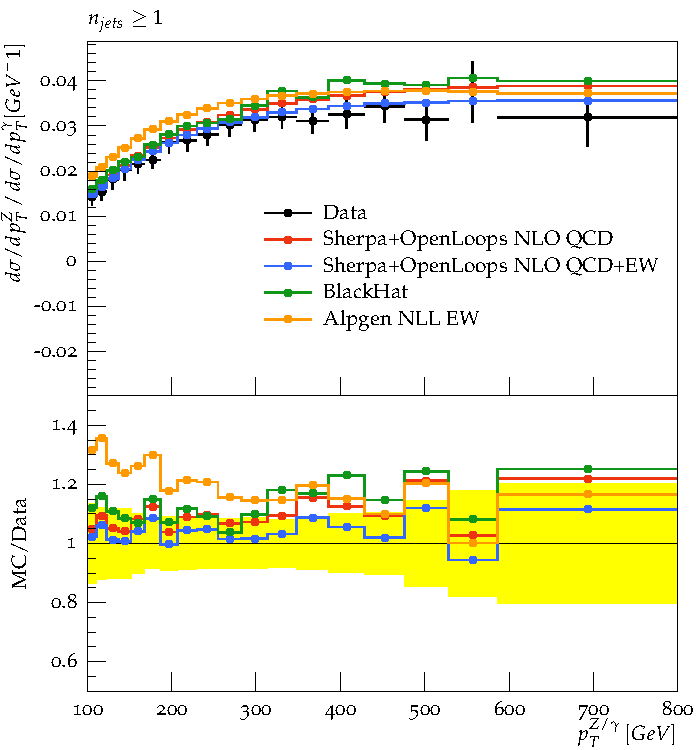
\includegraphics[width=0.6\textwidth]{Figure14.pdf} 
 \caption{Measurement of the ratio of Z + jets over $\gamma$ + jets at 8 TeV pp
   center-of-mass energy, in events with at least 1 jet accompanying the
   boson. Superimposed are shown different predictions at NLO QCD, next-leading-logs (NLL) EW and NLO QCD+EW order. 
   For fixed order predictions the number of jets corresponds to the
   number of partons in the final state at the lowest order.} 
\label{zgrNLO}
\end{center}
\end{figure}
The agreement of the combined NLO QCD+EW prediction with the CMS data is
remarkable over the whole spectrum. At low transverse momentum
NLO QCD corrections to the ratio are relevant due to mass effects, but sizable
EW corrections (of different size for the two processes) alter the shape of the ratio prediction already much below 1
TeV. These results show the importance of combining NLO QCD and EW corrections in a unified framework.

\section{Conclusions}

We reviewed the the most recent measurements of inclusive jet production, multi-jets production, jet properties and
photon and diphoton production in proton-proton collisions at the LHC. These measurements are important to test pQCD
predictions and constraint the PDF of the proton. The results that have been presented show that
event generators are in good agreement with the data. With the increase of the
centre-of-mass energy to 13 \TeV, however, there are hints that it will be necessary to include higher order QCD and EW
corrections to describe the data with the precision required by the high expected luminosity. 

\begin{thebibliography}{99}

\bibitem{Aad:2008zzm}
  G.~Aad {\it et al.} [ATLAS Collaboration],
  ``The ATLAS Experiment at the CERN Large Hadron Collider,''
  JINST {\bf 3} (2008) S08003.
  doi:10.1088/1748-0221/3/08/S08003

\bibitem{Chatrchyan:2008aa}
  S.~Chatrchyan {\it et al.} [CMS Collaboration],
  ``The CMS experiment at the CERN LHC,''
  JINST {\bf 3} (2008) S08004.
  doi:10.1088/1748-0221/3/08/S08004

\bibitem{Cacciari:2008gp}
  M.~Cacciari, G.~P.~Salam and G.~Soyez,
  ``The Anti-k(t) jet clustering algorithm,''
  JHEP {\bf 0804} (2008) 063
  doi:10.1088/1126-6708/2008/04/063
  [arXiv:0802.1189 [hep-ph]].

\bibitem{Lampl:2008zz} 
  W.~Lampl {\it et al.}, 
   ``Calorimeter clustering algorithms: Description and performance,''
  ATL-LARG-PUB-2008-002, ATL-COM-LARG-2008-003.

\bibitem{CMS:2009nxa}
  [CMS Collaboration],
  ``Particle-Flow Event Reconstruction in CMS and Performance for Jets, Taus, and MET,''
  CMS-PAS-PFT-09-001.

\bibitem{Khachatryan:2016wdh} 
  V.~Khachatryan {\it et al.} [CMS Collaboration], 
   ``Measurement of the double-differential inclusive jet cross section in proton-proton collisions at sqrt(s) = 13 TeV,'' 
  [arXiv:1605.04436 [hep-ex]]. 
   Submitted to: Eur.Phys.J.C.

\bibitem{Alioli:2010xa}
  S.~Alioli, K.~Hamilton, P.~Nason, C.~Oleari and E.~Re,
  ``Jet pair production in POWHEG,''
  JHEP {\bf 1104} (2011) 081
  doi:10.1007/JHEP04(2011)081
  [arXiv:1012.3380 [hep-ph]].

\bibitem{Sjostrand:2007gs}
  T.~Sjostrand, S.~Mrenna and P.~Z.~Skands,
  ``A Brief Introduction to PYTHIA 8.1,''
  Comput.\ Phys.\ Commun.\  {\bf 178} (2008) 852
  doi:10.1016/j.cpc.2008.01.036
  [arXiv:0710.3820 [hep-ph]].

\bibitem{Nagy:2003tz}
  Z.~Nagy,
  ``Next-to-leading order calculation of three jet observables in hadron hadron collision,''
  Phys.\ Rev.\ D {\bf 68} (2003) 094002
  doi:10.1103/PhysRevD.68.094002
  [hep-ph/0307268].

\bibitem{Dulat:2015mca}
  S.~Dulat {\it et al.},
  ``New parton distribution functions from a global analysis of quantum chromodynamics,''
  Phys.\ Rev.\ D {\bf 93} (2016) no.3,  033006
  doi:10.1103/PhysRevD.93.033006
  [arXiv:1506.07443 [hep-ph]].

\bibitem{CMS:2015haa}
  CMS Collaboration [CMS Collaboration],
  ``Measurement of the double-differential inclusive jet cross section at sqrt(s) = 8 TeV,''
  CMS-PAS-SMP-14-001.

\bibitem{Khachatryan:2015luy}
  V.~Khachatryan {\it et al.} [CMS Collaboration],
  ``Measurement of the inclusive jet cross section in pp collisions at $\sqrt{s} = 2.76\,\text {TeV}$,''
  Eur.\ Phys.\ J.\ C {\bf 76} (2016) no.5,  265
  doi:10.1140/epjc/s10052-016-4083-z
  [arXiv:1512.06212 [hep-ex]].

\bibitem{Abramowicz:2015mha}
  H.~Abramowicz {\it et al.} [H1 and ZEUS Collaborations],
  %``Combination of measurements of inclusive deep inelastic ${e^{\pm }p}$ scattering cross sections and QCD analysis of HERA data,''
  Eur.\ Phys.\ J.\ C {\bf 75} (2015) no.12,  580
  doi:10.1140/epjc/s10052-015-3710-4
  [arXiv:1506.06042 [hep-ex]].

\bibitem{Aaron:2009aa}
  F.~D.~Aaron {\it et al.} [H1 and ZEUS Collaborations],
  %``Combined Measurement and QCD Analysis of the Inclusive e+- p Scattering Cross Sections at HERA,''
  JHEP {\bf 1001} (2010) 109
  doi:10.1007/JHEP01(2010)109
  [arXiv:0911.0884 [hep-ex]].

\bibitem{Lai:2010vv}
  H.~L.~Lai, M.~Guzzi, J.~Huston, Z.~Li, P.~M.~Nadolsky, J.~Pumplin and C.-P.~Yuan,
  ``New parton distributions for collider physics,''
  Phys.\ Rev.\ D {\bf 82} (2010) 074024
  doi:10.1103/PhysRevD.82.074024
  [arXiv:1007.2241 [hep-ph]].

\bibitem{Agashe:2014kda}
  K.~A.~Olive {\it et al.} [Particle Data Group Collaboration],
  ``Review of Particle Physics,''
  Chin.\ Phys.\ C {\bf 38} (2014) 090001.
  doi:10.1088/1674-1137/38/9/090001

\bibitem{ATLAS:2015yaa}
  G.~Aad {\it et al.} [ATLAS Collaboration],
  ``Measurement of transverse energy-energy correlations in multi-jet events in $pp$ collisions at $\sqrt{s} = 7$ TeV using the ATLAS detector and determination of the strong coupling constant $\alpha_{\mathrm{s}}(m_Z)$,''
  Phys.\ Lett.\ B {\bf 750} (2015) 427
  doi:10.1016/j.physletb.2015.09.050
  [arXiv:1508.01579 [hep-ex]]. 

\bibitem{Aad:2015nda}
  G.~Aad {\it et al.} [ATLAS Collaboration],
  ``Measurement of four-jet differential cross sections in $\sqrt{s}=8$ TeV proton-proton collisions using the ATLAS detector,''
  JHEP {\bf 1512} (2015) 105
  doi:10.1007/JHEP12(2015)105
  [arXiv:1509.07335 [hep-ex]].

\bibitem{Berger:2008sj}
  C.~F.~Berger, Z.~Bern, L.~J.~Dixon, F.~Febres Cordero, D.~Forde, H.~Ita, D.~A.~Kosower and D.~Maitre,
  ``An Automated Implementation of On-Shell Methods for One-Loop Amplitudes,''
  Phys.\ Rev.\ D {\bf 78} (2008) 036003
  doi:10.1103/PhysRevD.78.036003
  [arXiv:0803.4180 [hep-ph]].

\bibitem{Bern:2011ep}
  Z.~Bern {\it et al.},
  ``Four-Jet Production at the Large Hadron Collider at Next-to-Leading Order in QCD,''
  Phys.\ Rev.\ Lett.\  {\bf 109} (2012) 042001
  doi:10.1103/PhysRevLett.109.042001
  [arXiv:1112.3940 [hep-ph]].

\bibitem{Badger:2012pg}
  S.~Badger, B.~Biedermann, P.~Uwer and V.~Yundin,
  ``Numerical evaluation of virtual corrections to multi-jet production in massless QCD,''
  Comput.\ Phys.\ Commun.\  {\bf 184} (2013) 1981
  doi:10.1016/j.cpc.2013.03.018
  [arXiv:1209.0100 [hep-ph]].

\bibitem{Badger:2012pf}
  S.~Badger, B.~Biedermann, P.~Uwer and V.~Yundin,
  ``NLO QCD corrections to multi-jet production at the LHC with a centre-of-mass energy of $\sqrt{s}=8$ TeV,''
  Phys.\ Lett.\ B {\bf 718} (2013) 965
  doi:10.1016/j.physletb.2012.11.029
  [arXiv:1209.0098 [hep-ph]].

\bibitem{Andersen:2009nu}
  J.~R.~Andersen and J.~M.~Smillie,
  ``Constructing All-Order Corrections to Multi-Jet Rates,''
  JHEP {\bf 1001} (2010) 039
  doi:10.1007/JHEP01(2010)039
  [arXiv:0908.2786 [hep-ph]].

\bibitem{Andersen:2011hs}
  J.~R.~Andersen and J.~M.~Smillie,
  ``Multiple Jets at the LHC with High Energy Jets,''
  JHEP {\bf 1106} (2011) 010
  doi:10.1007/JHEP06(2011)010
  [arXiv:1101.5394 [hep-ph]].

\bibitem{Alwall:2014hca}
  J.~Alwall {\it et al.},
  ``The automated computation of tree-level and next-to-leading order differential cross sections, and their matching to parton shower simulations,''
  JHEP {\bf 1407} (2014) 079
  doi:10.1007/JHEP07(2014)079
  [arXiv:1405.0301 [hep-ph]].

\bibitem{Sjostrand:2006za}
  T.~Sjostrand, S.~Mrenna and P.~Z.~Skands,
  ``PYTHIA 6.4 Physics and Manual,''
  JHEP {\bf 0605} (2006) 026
  doi:10.1088/1126-6708/2006/05/026
  [hep-ph/0603175].

\bibitem{Bahr:2008pv}
  M.~Bahr {\it et al.},
  ``Herwig++ Physics and Manual,''
  Eur.\ Phys.\ J.\ C {\bf 58} (2008) 639
  doi:10.1140/epjc/s10052-008-0798-9
  [arXiv:0803.0883 [hep-ph]].

 \bibitem{Khachatryan:2016udy}
  V.~Khachatryan {\it et al.} [CMS Collaboration],
  ``Azimuthal decorrelation of jets widely separated in rapidity in pp collisions at $\sqrt{s} =$ 7 TeV,''
  Submitted to: JHEP
  [arXiv:1601.06713 [hep-ex]].

\bibitem{Khachatryan:2015xwa}
  V.~Khachatryan {\it et al.} [CMS Collaboration],
  ``Distributions of Topological Observables in Inclusive Three- and Four-Jet Events in pp Collisions at sqrt(s) = 7 TeV,''
  Eur.\ Phys.\ J.\ C {\bf 75} (2015) no.7,  302
  doi:10.1140/epjc/s10052-015-3491-9
  [arXiv:1502.04785 [hep-ex]].

\bibitem{Khachatryan:2016hkr}
  V.~Khachatryan {\it et al.} [CMS Collaboration],
  ``Measurement of dijet azimuthal decorrelation in pp collisions at $\sqrt{s}$ = 8 TeV,''
  Submitted to: Eur.Phys.J.C
  [arXiv:1602.04384 [hep-ex]].

\bibitem{Aad:2016oit}
  G.~Aad {\it et al.} [ATLAS Collaboration],
  ``Measurement of the charged-particle multiplicity inside jets from $\sqrt{s}=8$ TeV $pp$ collisions with the ATLAS detector,''
  Eur.\ Phys.\ J.\ C {\bf 76} (2016) no.6,  322
  doi:10.1140/epjc/s10052-016-4126-5
  [arXiv:1602.00988 [hep-ex]].

\bibitem{Aad:2015cua}
  G.~Aad {\it et al.} [ATLAS Collaboration],
  ``Measurement of jet charge in dijet events from $\sqrt{s}$=8  TeV pp collisions with the ATLAS detector,''
  Phys.\ Rev.\ D {\bf 93} (2016) no.5,  052003
  doi:10.1103/PhysRevD.93.052003
  [arXiv:1509.05190 [hep-ex]].

\bibitem{CMS:2016yuu}
  CMS Collaboration [CMS Collaboration],
  ``Measurement of jet charge observables in dijet events at $\sqrt{s}=8~\mathrm{TeV}$,''
  CMS-PAS-SMP-15-003.

\bibitem{Pumplin:2002vw}
  J.~Pumplin, D.~R.~Stump, J.~Huston, H.~L.~Lai, P.~M.~Nadolsky and W.~K.~Tung,
  ``New generation of parton distributions with uncertainties from global QCD analysis,''
  JHEP {\bf 0207} (2002) 012
  doi:10.1088/1126-6708/2002/07/012
  [hep-ph/0201195].

\bibitem{ATLAS:2012ana}
  [ATLAS Collaboration],
  ``Measurements of the photon identification efficiency with the ATLAS detector using 4.9 fb−1 of pp collision data collected in 2011,''
  ATLAS-CONF-2012-123.

\bibitem{Chatrchyan:2013dga}
  S.~Chatrchyan {\it et al.} [CMS Collaboration],
  ``Energy Calibration and Resolution of the CMS Electromagnetic Calorimeter in $pp$ Collisions at $\sqrt{s} = 7$ TeV,''
  JINST {\bf 8} (2013) P09009
   [JINST {\bf 8} (2013) 9009]
  doi:10.1088/1748-0221/8/09/P09009
  [arXiv:1306.2016 [hep-ex]].

\bibitem{Aad:2016xcr}
  G.~Aad {\it et al.} [ATLAS Collaboration],
  ``Measurement of the inclusive isolated prompt photon cross section in pp collisions at $ \sqrt{s}=8 $ TeV with the ATLAS detector,''
  JHEP {\bf 1608} (2016) 005
  doi:10.1007/JHEP08(2016)005
  [arXiv:1605.03495 [hep-ex]].

\bibitem{Catani:2002ny}
  S.~Catani, M.~Fontannaz, J.~P.~Guillet and E.~Pilon,
  ``Cross-section of isolated prompt photons in hadron hadron collisions,''
  JHEP {\bf 0205} (2002) 028
  doi:10.1088/1126-6708/2002/05/028
  [hep-ph/0204023].

\bibitem{CMS:2015hha}
  CMS Collaboration [CMS Collaboration],
  ``Production of pairs of isolated photons in association with jets in pp collisions at sqrt(s) = 7 TeV,''
  CMS-PAS-SMP-14-021.

\bibitem{Gehrmann:2013aga}
  T.~Gehrmann, N.~Greiner and G.~Heinrich,
  ``Photon isolation effects at NLO in $\gamma \gamma$ + jet final states in hadronic collisions,''
  JHEP {\bf 1306} (2013) 058
   Erratum: [JHEP {\bf 1406} (2014) 076]
  doi:10.1007/JHEP06(2014)076, 10.1007/JHEP06(2013)058
  [arXiv:1303.0824 [hep-ph]].

\bibitem{Chatrchyan:2014fsa}
  S.~Chatrchyan {\it et al.} [CMS Collaboration],
  ``Measurement of differential cross sections for the production of a pair of isolated photons in pp collisions at $\sqrt{s}=7\,\text {TeV} $,''
  Eur.\ Phys.\ J.\ C {\bf 74} (2014) no.11,  3129
  doi:10.1140/epjc/s10052-014-3129-3
  [arXiv:1405.7225 [hep-ex]].

\bibitem{Khachatryan:2015ira}
  V.~Khachatryan {\it et al.} [CMS Collaboration],
  %``Comparison of the Z/$\gamma$$^{∗}$ + jets to $\gamma$ + jets cross sections in pp collisions at $ \sqrt{s}=8 $ TeV,''
  JHEP {\bf 1510} (2015) 128
   Erratum: [JHEP {\bf 1604} (2016) 010]
  doi:10.1007/JHEP04(2016)010, 10.1007/JHEP10(2015)128
  [arXiv:1505.06520 [hep-ex]].

\bibitem{Kallweit:2014xda}
  S.~Kallweit, J.~M.~Lindert, P.~Maierhöfer, S.~Pozzorini and M.~Schönherr,
  ``NLO electroweak automation and precise predictions for W+multijet production at the LHC,''
  JHEP {\bf 1504} (2015) 012
  doi:10.1007/JHEP04(2015)012
  [arXiv:1412.5157 [hep-ph]].

\bibitem{Kallweit:2015dum}
  S.~Kallweit, J.~M.~Lindert, P.~Maierhofer, S.~Pozzorini and M.~Schönherr,
  ``NLO QCD+EW predictions for V + jets including off-shell vector-boson decays and multijet merging,''
  JHEP {\bf 1604} (2016) 021
  doi:10.1007/JHEP04(2016)021
  [arXiv:1511.08692 [hep-ph]].

\end{thebibliography}

\end{document}
